\chapter{fundamentação teórica}
\label{cap:fundamentacao-teorica}



% ==============================================================================
% FUNDAMENTAÇÃO TEÓRICA — Pré-processamento de sinais de ECG
%
% Conceitos gerais. Os valores específicos adotados neste trabalho estão na
% metodologia (metodologia_preprocessamento.tex).
% ==============================================================================

\section{Pré-processamento de sinais eletrocardiográficos}
\label{sec:fund-preprocessamento}

O sinal registrado pelo eletrocardiógrafo contém, além da atividade
elétrica cardíaca, componentes de origem diversa que se sobrepõem a ela. O
pré-processamento tem por objetivo atenuar esses componentes preservando a
morfologia das ondas de interesse, e a escolha de seus parâmetros resulta de
um compromisso entre remover ruído e não distorcer o sinal
\cite{clifford2006advanced}.

\subsection{Fontes de interferência}
\label{subsec:fund-ruidos}

Três fontes de interferência predominam no registro ambulatorial.

A \textit{oscilação da linha de base} consiste em variações lentas do nível
do sinal, provocadas pela respiração, pela movimentação do paciente e pela
alteração da impedância na interface entre eletrodo e pele. Seu conteúdo
espectral concentra-se abaixo de 0,5\,Hz, e seu efeito é deslocar o traçado
verticalmente ao longo do tempo, dificultando a comparação de amplitudes
entre batimentos.

A \textit{interferência da rede elétrica} manifesta-se como componente
senoidal na frequência de alimentação --- 50\,Hz na Europa, onde foi
adquirida a base empregada neste trabalho --- e em seus harmônicos.

O \textit{ruído muscular}, decorrente da atividade elétrica dos músculos
esqueléticos, ocupa banda larga, predominantemente acima de 20\,Hz. No
Holter, ao qual o paciente permanece conectado durante suas atividades
habituais, esse ruído é mais frequente que no exame de repouso, e se soma aos
\textit{artefatos de movimento} produzidos pelo deslocamento dos eletrodos.

A energia do próprio \gls{ECG}, por sua vez, concentra-se em faixa
relativamente estreita. As ondas P e T, de evolução lenta, ocupam
predominantemente frequências abaixo de 10\,Hz; o complexo QRS, de
transição rápida, estende-se até algumas dezenas de hertz. Essa separação
parcial entre o conteúdo do sinal e o das interferências é o que torna a
filtragem por faixa de frequência eficaz.

\subsection{Filtragem digital}
\label{subsec:fund-filtragem}

Um filtro passa-faixa atenua as componentes situadas abaixo de uma
frequência de corte inferior $f_{\mathrm{inf}}$ e acima de uma frequência de
corte superior $f_{\mathrm{sup}}$, preservando a faixa intermediária. A
escolha de $f_{\mathrm{inf}}$ determina quanto da oscilação de linha de base é
removida; a de $f_{\mathrm{sup}}$, quanto do ruído muscular e da interferência
da rede.

As recomendações da American Heart Association para o \gls{ECG} diagnóstico
estabelecem frequência de corte inferior de 0,05\,Hz para filtros
convencionais, admitindo até 0,67\,Hz quando o filtro digital não introduz
distorção de fase \cite{kligfield2007recommendations}. A ressalva decorre de
que filtros com resposta de fase não linear deslocam componentes de
frequências distintas por intervalos de tempo diferentes, o que distorce
segmentos de evolução lenta, como o segmento ST.

\subsubsection{Filtro de Butterworth}
\label{subsubsec:fund-butterworth}

O filtro de Butterworth \cite{butterworth1930theory} caracteriza-se por
resposta em magnitude maximamente plana na banda passante. Para um filtro
passa-baixas de ordem $n$ e frequência de corte $f_c$, a magnitude da
resposta em frequência é

\begin{equation}
	|H(f)| = \frac{1}{\sqrt{1 + (f / f_c)^{2n}}}.
	\label{eq:butterworth}
\end{equation}

A ausência de ondulações na banda passante preserva a amplitude relativa das
componentes do sinal, propriedade desejável quando a morfologia das ondas é a
informação de interesse. A ordem $n$ controla a inclinação da transição entre
as bandas passante e de rejeição: ordens maiores produzem corte mais abrupto,
ao custo de maior atraso e maior sensibilidade numérica. A implementação em
seções de segunda ordem em cascata contorna essa sensibilidade, decompondo o
filtro em blocos de baixa ordem numericamente estáveis.

\subsubsection{Filtragem de fase nula}
\label{subsubsec:fund-fase-nula}

A filtragem direta e reversa aplica o mesmo filtro duas vezes: primeiro no
sentido temporal e, em seguida, sobre o sinal invertido no tempo
\cite{gustafsson1996determining}. O atraso de fase introduzido na primeira
passagem é exatamente compensado pela segunda, de modo que o resultado não
apresenta distorção de fase. A magnitude da resposta, por sua vez, é elevada
ao quadrado, o que equivale a dobrar a ordem efetiva do filtro.

A operação não é causal, pois a saída em cada instante depende de amostras
futuras. Essa restrição impede seu uso em monitoramento em tempo real, mas não
representa limitação na análise de registros já adquiridos, como é o caso do
Holter.

\subsection{Normalização de amplitude}
\label{subsec:fund-normalizacao}

Redes neurais são sensíveis à escala da entrada: valores de magnitudes muito
distintas entre exemplos dificultam a otimização. Duas estratégias de
normalização são usuais em sinais, e diferem quanto à informação que
preservam.

A \textit{padronização por segmento} subtrai a média e divide pelo
desvio-padrão de cada trecho individualmente. Todos os segmentos passam a ter
média nula e variância unitária, independentemente da amplitude original. A
estratégia é robusta a diferenças de ganho entre equipamentos, mas elimina a
informação de amplitude absoluta --- um traçado de baixa voltagem e outro de
alta voltagem tornam-se indistinguíveis quanto à escala.

A \textit{normalização por escala global} divide todos os segmentos por uma
mesma constante, estimada sobre o conjunto de treinamento. A amplitude
relativa entre pacientes é preservada, o que é relevante no \gls{ECG}: a baixa
voltagem e a hipertrofia ventricular manifestam-se justamente como amplitudes
anormalmente reduzidas ou elevadas. A estimativa da constante por percentil
elevado do valor absoluto, em lugar do máximo, confere robustez a artefatos
pontuais de grande amplitude.

\subsection{Amostragem em janelas e independência entre exemplos}
\label{subsec:fund-janelas}

Registros de longa duração raramente são processados integralmente por redes
neurais, em razão do volume de memória envolvido: 24\,horas a 200\,Hz em três
derivações correspondem a aproximadamente 17 milhões de amostras. A prática
usual consiste em extrair janelas de duração fixa, cada uma tratada como
exemplo de treinamento.

Essa estratégia introduz uma dependência entre exemplos que tem consequências
metodológicas. Janelas de um mesmo paciente compartilham características
individuais estáveis --- eixo elétrico, morfologia do complexo QRS, relação de
amplitude entre derivações ---, e não constituem observações independentes.
Se janelas de um mesmo indivíduo forem distribuídas entre os conjuntos de
treinamento e teste, o modelo pode reconhecer o paciente em lugar de estimar
o desfecho, produzindo estimativas de desempenho otimistas. Esse tipo de
vazamento de informação está entre as causas mais frequentes de resultados
não reprodutíveis em aprendizado de máquina aplicado
\cite{kapoor2023leakage}. A prevenção exige que a divisão entre conjuntos seja
realizada no nível do paciente, e que as métricas sejam calculadas após a
agregação das predições de suas janelas.


% ==============================================================================
% FUNDAMENTAÇÃO TEÓRICA — Redes neurais convolucionais unidimensionais
% Baseado em cnn_classificacao.py
%
% Estrutura:
%   1. Conceitos comuns a todas as arquiteturas (convolução, ativação,
%      normalização, agrupamento, descarte, função de perda)
%   2. A rede convolucional empregada neste trabalho
%
% As seções seguintes (ResNet, atenção, LSTM, DeepHHF, MIL) remetem aos
% conceitos definidos aqui, evitando repetição.
%
% Notação: conforme notacao_dissertacao.md
%   S  sinal (C x L)     C derivações     L comprimento     kappa  núcleo
%   sigma(.) logística   w_+ peso da classe positiva   theta parâmetros
% ==============================================================================

\section{Redes neurais convolucionais unidimensionais}
\label{sec:fund-cnn}

As redes neurais convolucionais (CNN)\glsadd{CNN}\glsunset{CNN} foram concebidas para dados com estrutura
espacial ou temporal, nos quais elementos próximos guardam relação entre si
\cite{lecun1998gradient}. Embora popularizadas no processamento de imagens,
sua formulação unidimensional aplica-se diretamente a sinais fisiológicos,
nos quais a vizinhança temporal carrega a informação relevante
\cite{kiranyaz2021onedimensional}. No \gls{ECG}, a morfologia de cada onda
é definida pela sucessão de amostras ao longo de algumas dezenas de
milissegundos, e é essa estrutura local que a convolução explora.

Esta seção apresenta inicialmente as operações que compõem as arquiteturas
avaliadas neste trabalho e, em seguida, descreve a rede convolucional
empregada como primeira abordagem.

\subsection{Convolução unidimensional}
\label{subsec:fund-convolucao}

Seja $\mathbf{S} \in \mathbb{R}^{C \times L}$ um sinal com $C$ derivações e
$L$ amostras. Uma camada convolucional unidimensional aplica $C'$ filtros,
cada um definido por um núcleo $\boldsymbol{\Theta}_{c'} \in
	\mathbb{R}^{C \times \kappa}$ de largura $\kappa$. A saída do filtro $c'$ na
posição $t$ é dada por

\begin{equation}
	h_{c'}(t) = b_{c'} + \sum_{c=1}^{C} \sum_{j=0}^{\kappa-1}
	\Theta_{c',c,j} \; S_{c}\!\left(t + j - \left\lfloor \kappa/2 \right\rfloor\right),
	\label{eq:convolucao}
\end{equation}

\noindent
em que $b_{c'}$ é um termo de viés. O filtro percorre o sinal posição a
posição, e em cada uma combina os $\kappa$ valores vizinhos de todas as
derivações em um único número. Valores elevados indicam que o trecho
analisado se assemelha ao padrão codificado no filtro.

Duas propriedades tornam a operação adequada a sinais. A primeira é o
\textit{compartilhamento de pesos}: o mesmo núcleo é aplicado em todas as
posições, de modo que um padrão aprendido em um instante é reconhecido em
qualquer outro. A segunda é a \textit{conectividade local}: cada saída
depende apenas de $\kappa$ amostras vizinhas, o que reduz drasticamente o
número de parâmetros em relação a uma camada totalmente conectada. Uma
camada com $C$ entradas, $C'$ filtros e núcleo $\kappa$ possui
$C \cdot C' \cdot \kappa$ pesos, independentemente do comprimento $L$ do
sinal.

O preenchimento de $\lfloor \kappa/2 \rfloor$ amostras nas extremidades
preserva o comprimento da saída. A largura do núcleo, por sua vez, determina
a escala temporal dos padrões que cada filtro é capaz de representar
isoladamente.

\subsection{Função de ativação}
\label{subsec:fund-ativacao}

A composição de operações lineares resulta em operação linear, de modo que
empilhar camadas convolucionais sem não linearidades intermediárias não
aumentaria a capacidade de representação do modelo. Emprega-se, por isso, a
função de ativação retificada linear \cite{nair2010rectified}:

\begin{equation}
	\mathrm{ReLU}(z) = \max(0, z).
	\label{eq:relu}
\end{equation}

A função anula valores negativos e preserva os positivos. Em termos
interpretativos, cada filtro passa a indicar a presença do padrão
correspondente, e não sua ausência. Do ponto de vista da otimização, sua
derivada unitária na região positiva evita a atenuação do gradiente que
afeta funções saturantes, como a tangente hiperbólica.

\subsection{Normalização em lote}
\label{subsec:fund-batchnorm}

À medida que os parâmetros de uma camada se alteram durante o treinamento, a
distribuição de suas saídas também se altera, o que obriga as camadas
seguintes a se readaptarem continuamente. A normalização em lote
\cite{ioffe2015batch} atenua esse efeito padronizando cada canal com a
média $\mu_{\mathcal{B}}$ e a variância $\sigma^{2}_{\mathcal{B}}$
calculadas sobre o lote $\mathcal{B}$:

\begin{equation}
	\hat{h} = \gamma \, \frac{h - \mu_{\mathcal{B}}}
	{\sqrt{\sigma^{2}_{\mathcal{B}} + \epsilon}} + \beta,
	\label{eq:batchnorm}
\end{equation}

\noindent
em que $\gamma$ e $\beta$ são parâmetros aprendidos que permitem à rede
recuperar a escala original, caso seja conveniente, e $\epsilon$ é uma
constante de estabilidade numérica. Durante a avaliação, $\mu_{\mathcal{B}}$
e $\sigma^{2}_{\mathcal{B}}$ são substituídas por médias móveis acumuladas no
treinamento, de modo que a predição de um paciente não dependa dos demais
presentes no mesmo lote.

\subsection{Agrupamento}
\label{subsec:fund-pooling}

O agrupamento máximo com fator $r$ divide a sequência em trechos de $r$
posições e retém apenas o maior valor de cada um, reduzindo o comprimento por
esse fator. A operação tem dois efeitos. O primeiro é a redução do custo
computacional das camadas seguintes. O segundo é a ampliação progressiva da
escala temporal: após o agrupamento, cada posição resume $r$ amostras da
camada anterior, e a convolução seguinte, com o mesmo núcleo $\kappa$, passa
a abranger trecho $r$ vezes mais longo do sinal original.

Ao término da sequência de camadas convolucionais, o agrupamento global
colapsa integralmente o eixo temporal \cite{lin2014network}. O agrupamento
global por média produz, para cada canal, o valor médio ao longo da janela;
o agrupamento global máximo, o valor no instante de maior ativação:

\begin{equation}
	z_{c}^{\text{méd}} = \frac{1}{L'} \sum_{t=1}^{L'} h_{c}(t),
	\qquad
	z_{c}^{\text{máx}} = \max_{t} \, h_{c}(t),
	\label{eq:pooling-global}
\end{equation}

\noindent
em que $L'$ é o comprimento da sequência após as camadas convolucionais. A
representação resultante tem dimensão fixa, independente do comprimento da
entrada, o que permite à mesma rede processar janelas de durações distintas.

\subsection{Descarte}
\label{subsec:fund-dropout}

O descarte (\textit{dropout}) anula aleatoriamente uma fração $p$ das
unidades a cada passo de treinamento \cite{srivastava2014dropout}. Como
nenhuma unidade pode contar com a presença das demais, a rede é impelida a
distribuir a informação entre múltiplos caminhos redundantes, o que reduz a
tendência de memorizar exemplos específicos. Na avaliação, todas as unidades
são mantidas e suas saídas, escaladas pelo fator correspondente.

\subsection{Função de perda e desbalanceamento}
\label{subsec:fund-perda}

A rede produz, para cada exemplo $i$, um valor real $z_i$ denominado
\textit{logit}, convertido em probabilidade pela função logística:

\begin{equation}
	\hat{p}_i = \sigma(z_i) = \frac{1}{1 + \mathrm{e}^{-z_i}}.
	\label{eq:logistica}
\end{equation}

O ajuste dos parâmetros $\theta$ minimiza a entropia cruzada binária. Em
problemas com classes desbalanceadas, a contribuição dos exemplos positivos
é multiplicada por um peso $w_{+}$:

\begin{equation}
	\mathcal{L}(\theta) = -\frac{1}{B} \sum_{i=1}^{B}
	\Big[\, w_{+}\, y_i \log \hat{p}_i + (1 - y_i) \log(1 - \hat{p}_i) \Big],
	\label{eq:bce-ponderada}
\end{equation}

\noindent
em que $B$ é o tamanho do lote e $y_i \in \{0, 1\}$ o rótulo. Sem a
ponderação, a perda poderia ser minimizada atribuindo-se a classe
majoritária a todos os exemplos --- solução que, com prevalência de
10,6\,\%, alcança acurácia de 89,4\,\% com sensibilidade nula. A escolha
$w_{+} = N_0/N_1$, razão entre o número de exemplos negativos e positivos,
torna a contribuição total das duas classes equivalente, o que corresponde a
replicar cada exemplo positivo $w_{+}$ vezes sem descartar exemplos
negativos.

A minimização emprega o otimizador AdamW \cite{loshchilov2019decoupled}, que
adapta a taxa de aprendizado de cada parâmetro à magnitude histórica de seus
gradientes e aplica a regularização por decaimento de pesos de forma
desacoplada da atualização do gradiente.

% ==============================================================================

\subsection{Arquitetura empregada}
\label{subsec:fund-cnn-arquitetura}

A rede convolucional adotada neste trabalho é composta por blocos
sequenciais, seguidos de agrupamento global e de um classificador de duas
camadas. Cada bloco aplica, nesta ordem, convolução, normalização em lote,
ativação \textit{ReLU}, agrupamento máximo com fator quatro e descarte com
probabilidade 0,1. A \autoref{fig:cnn-arquitetura} ilustra o fluxo.

% ---- FIGURA: diagrama da arquitetura ----
\begin{figure}[h!]
	\captionsetup{width=16cm}
	\Caption{\label{fig:cnn-arquitetura} Arquitetura da rede convolucional
		unidimensional}
	\UFCfig{}{
		\fbox{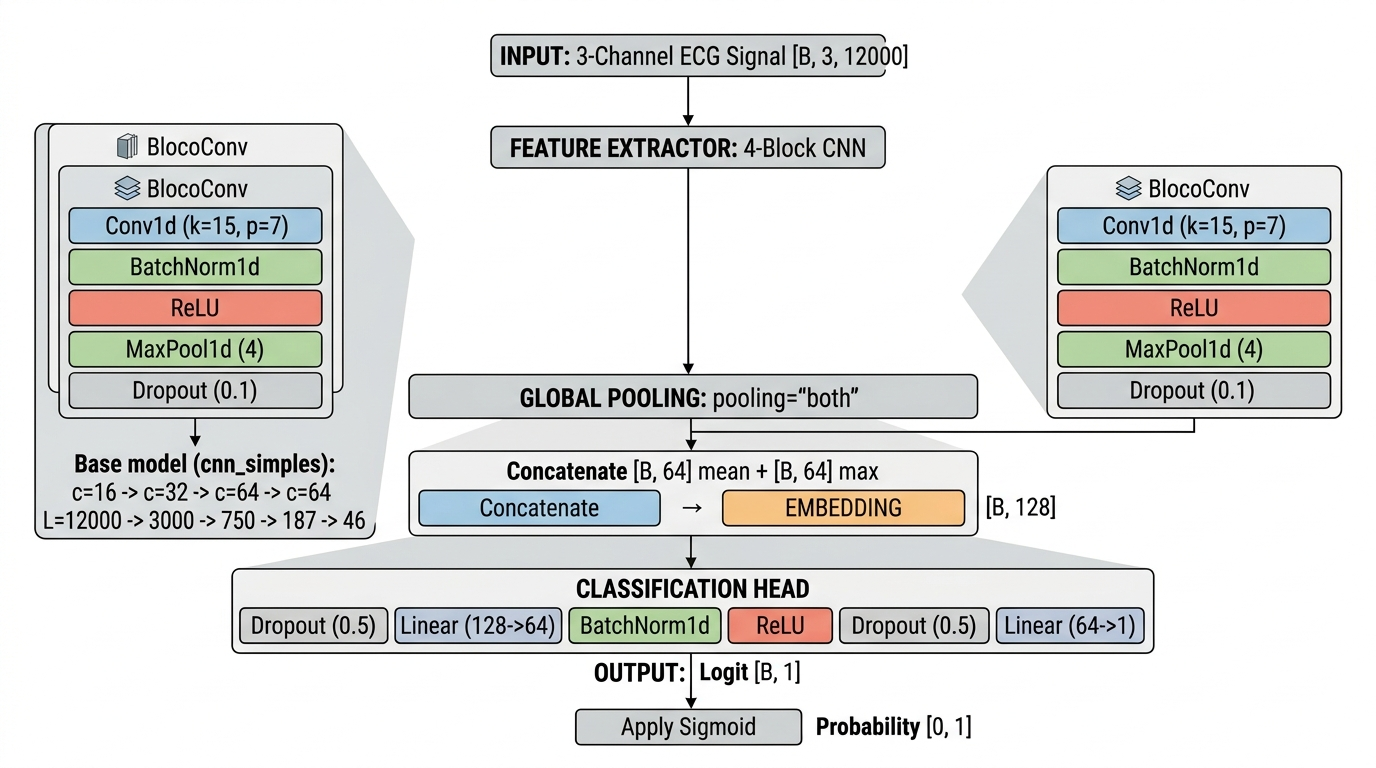
\includegraphics[width=16cm]{figuras/arquitetura_cnn.jpg}}
	}{
		\Fonte{elaborado pelo autor (2026).}
	}
\end{figure}

\subsubsection{Variantes de capacidade}
\label{subsubsec:fund-cnn-variantes}

Para avaliar se o desempenho depende da capacidade do modelo, a mesma
estrutura foi instanciada em três tamanhos, que diferem apenas no número de
blocos e de filtros por bloco. A variante \textit{mínima} tem três blocos,
com 8, 16 e 32 filtros; a \textit{simples}, quatro blocos, com 16, 32, 64 e
64 filtros; a \textit{média}, quatro blocos, com 32, 64, 128 e 128 filtros.
Todos os demais elementos --- largura do núcleo, agrupamento, descarte,
classificador e inicialização --- são idênticos. Entre a menor e a maior
variante, o número de parâmetros cresce cerca de 29 vezes. Se o desempenho
não acompanhar esse crescimento, a limitação não está na capacidade da
rede, mas na informação disponível nos dados.

A \autoref{tab:cnn-dimensoes} detalha os canais de cada variante e o
comprimento das representações intermediárias para as duas durações de
janela avaliadas: 2~minutos (24\,000 amostras) e 10~segundos (2\,000
amostras).

% ---- TABELA: dimensões ----
\begin{table}[h!]
	\captionsetup{width=15.5cm}
	\Caption{\label{tab:cnn-dimensoes} Canais e comprimento das
		representações intermediárias das variantes da rede convolucional}
	\IBGEtab{}{
		\begin{tabular}{lrrrrrr}
			\toprule
			                          & \multicolumn{3}{c}{Canais}          & \multicolumn{2}{c}{Comprimento} &                                         \\
			\cmidrule(lr){2-4} \cmidrule(lr){5-6}
			Etapa                     & \multicolumn{1}{c}{Mínima}          & \multicolumn{1}{c}{Simples}     &
			\multicolumn{1}{c}{Média} & \multicolumn{1}{c}{2 min}           &
			\multicolumn{1}{c}{10 s}  & \multicolumn{1}{c}{Campo receptivo}                                                                             \\
			\midrule \midrule
			Entrada                   & 3                                   & 3                               & 3   & 24\,000 & 2\,000 & 5\,ms          \\
			Bloco 1                   & 8                                   & 16                              & 32  & 6\,000  & 500    & 90\,ms         \\
			Bloco 2                   & 16                                  & 32                              & 64  & 1\,500  & 125    & 430\,ms        \\
			Bloco 3                   & 32                                  & 64                              & 128 & 375     & 31     & 1,8\,s         \\
			Bloco 4                   & ---                                 & 64                              & 128 & 93      & 7      & 7,2\,s         \\
			Agrupamento global        & 64                                  & 128                             & 256 & ---     & ---    & janela inteira \\
			\bottomrule
		\end{tabular}
	}{
		\Fonte{elaborado pelo autor (2026).}
	}
\end{table}

A coluna de campo receptivo indica a extensão do sinal original que
influencia cada posição de saída e não depende da duração da janela. Ao
final do primeiro bloco, cada posição reflete 90\,ms de registro ---
aproximadamente a duração de um complexo QRS ---; ao final do quarto,
7,2\,s, o equivalente a oito a nove ciclos cardíacos a 70\,bpm. A rede,
portanto, combina progressivamente padrões morfológicos de batimentos
isolados em padrões que abrangem sequências de batimentos.

A duração da janela altera o que esses padrões representam no conjunto.
Na janela de 2~minutos, o quarto bloco ainda produz 93 posições, cada uma
resumindo alguns segundos, e o agrupamento global combina dezenas de trechos
distintos. Na janela de 10~segundos, restam 7 posições cujo campo receptivo
já cobre a maior parte da janela, de modo que a rede analisa essencialmente
um único trecho de poucos batimentos. Na variante mínima, que não possui o
quarto bloco, o campo receptivo final é de 1,8\,s, cerca de dois ciclos
cardíacos.

\subsubsection{Largura do núcleo}
\label{subsubsec:fund-cnn-nucleo}

O núcleo convolucional foi dimensionado em $\kappa = 15$ amostras,
equivalentes a 75\,ms na frequência de 200\,Hz. A escolha difere da convenção
predominante em arquiteturas originadas no processamento de imagens, em que
núcleos de três elementos são usuais e corresponderiam, neste contexto, a
apenas 15\,ms. Com núcleo de 75\,ms, um único filtro da primeira camada
abrange parcela substancial de um complexo QRS, cuja duração normal situa-se
entre 80 e 100\,ms, podendo representar diretamente padrões de despolarização
ventricular.

\subsubsection{Agrupamento combinado}
\label{subsubsec:fund-cnn-pooling}

Ao término do último bloco, os canais são reduzidos a um vetor com o dobro
da sua dimensão pela concatenação dos agrupamentos globais por média e
máximo, conforme a \autoref{eq:pooling-global}: 64, 128 e 256 dimensões nas
variantes mínima, simples e média. As duas operações capturam aspectos
complementares: a média reflete o comportamento típico da janela, enquanto o
máximo registra o instante de maior ativação de cada filtro. A combinação
permite que a rede seja sensível tanto a alterações persistentes quanto a
eventos breves, como extrassístoles isoladas, que a média isoladamente
diluiria.

\subsubsection{Ausência de conexões residuais}
\label{subsubsec:fund-cnn-residual}

A arquitetura não emprega as conexões residuais descritas na
\autoref{sec:fund-resnet}. Essas conexões foram concebidas para viabilizar o
treinamento de redes com dezenas de camadas, nas quais o gradiente tenderia a
se atenuar ao percorrer a sequência de transformações. Com três ou quatro
blocos convolucionais, o gradiente alcança as camadas iniciais sem atenuação
significativa, e os atalhos acrescentariam parâmetros sem benefício
correspondente.

\subsubsection{Classificador e número de parâmetros}
\label{subsubsec:fund-cnn-classificador}

O vetor resultante do agrupamento alimenta um classificador composto por
duas camadas totalmente conectadas --- a primeira com 64 unidades,
normalização em lote e ativação \textit{ReLU}, a segunda com uma unidade de
saída ---, ambas precedidas por descarte com probabilidade 0,6. Os pesos das
camadas convolucionais são inicializados conforme \citeonline{he2015delving},
esquema adequado a redes com ativação \textit{ReLU}.

A \autoref{tab:cnn-parametros} decompõe os parâmetros treináveis de cada
variante. Como as camadas convolucionais não dependem do comprimento do
sinal, os valores são os mesmos para as duas durações de janela.

% ---- TABELA: parâmetros ----
\begin{table}[h!]
	\captionsetup{width=13.5cm}
	\Caption{\label{tab:cnn-parametros} Distribuição dos parâmetros das
		variantes da rede convolucional}
	\IBGEtab{}{
		\begin{tabular}{lrrr}
			\toprule
			Componente                  & \multicolumn{1}{c}{Mínima} &
			\multicolumn{1}{c}{Simples} & \multicolumn{1}{c}{Média}                        \\
			\midrule \midrule
			Bloco 1                     & 360                        & 720      & 1\,440   \\
			Bloco 2                     & 1\,920                     & 7\,680   & 30\,720  \\
			Bloco 3                     & 7\,680                     & 30\,720  & 122\,880 \\
			Bloco 4                     & ---                        & 61\,440  & 245\,760 \\
			Normalização dos blocos     & 112                        & 352      & 704      \\
			Classificador               & 4\,353                     & 8\,449   & 16\,641  \\
			\midrule
			Total                       & 14\,425                    & 109\,361 & 418\,145 \\
			Por paciente de treino      & 47                         & 354      & 1\,353   \\
			\bottomrule
		\end{tabular}
	}{
		\Fonte{elaborado pelo autor (2026).}
	}
\end{table}

Cada bloco convolucional tem $C \cdot C' \cdot \kappa$ pesos, sem termo de
viés, pois a normalização em lote seguinte o tornaria redundante. A última
linha divide o total pelos 309 pacientes do conjunto de treinamento de cada
partição. Mesmo a variante média tem cerca de dez vezes menos parâmetros por
paciente que a ResNet-18 descrita na \autoref{sec:fund-resnet}, que tem 3\,976\,385
parâmetros, ou 12\,869 por paciente de treinamento.

% arquitetura resnet =======================================

% ==============================================================================
% FUNDAMENTAÇÃO TEÓRICA — Redes residuais
% Baseado em resnet_classificacao.py (classes BasicBlock1d, Bottleneck1d, ResNet1d)
%
% Cobre as quatro configurações avaliadas: ResNet-18 reduzida, ResNet-18
% completa, ResNet-34 e ResNet-50. A variante com camada de atenção
% (ResNetTransformer, no mesmo arquivo) é tratada na seção seguinte, pois
% introduz o mecanismo de atenção.
%
% Remete às operações definidas em fundamentacao_cnn.tex
% (eq:convolucao, eq:relu, eq:batchnorm, eq:pooling-global).
% ==============================================================================

\section{Redes neurais residuais}
\label{sec:fund-resnet}
\glsadd{ResNet}\glsunset{ResNet}%

A profundidade é um dos fatores que determinam a capacidade de
representação de uma rede neural: camadas sucessivas permitem compor padrões
simples em padrões progressivamente mais abstratos. Empiricamente, contudo,
o acréscimo de camadas a partir de certo ponto deixa de melhorar e passa a
piorar o desempenho --- não por sobreajuste, mas porque o próprio erro de
treinamento aumenta. \citeonline{he2016deep} denominaram esse fenômeno
\textit{problema de degradação} e propuseram as redes residuais como
solução.

\subsection{Aprendizado residual}
\label{subsec:fund-residual}

O argumento parte de uma construção. Uma rede mais profunda poderia, em
princípio, reproduzir o desempenho de uma rede rasa se as camadas
adicionais implementassem a função identidade. Que redes profundas não
alcancem sequer esse desempenho indica que aproximar a identidade por meio
de sucessivas transformações não lineares é difícil para os métodos de
otimização usuais.

A proposta consiste em reformular o que cada bloco aprende. Em lugar de
estimar diretamente o mapeamento desejado $\mathcal{H}(\mathbf{x})$, o bloco
estima o resíduo $\mathcal{F}(\mathbf{x}) = \mathcal{H}(\mathbf{x}) -
	\mathbf{x}$, e a saída é obtida somando-se a entrada de volta:

\begin{equation}
	\mathbf{y} = \mathcal{F}(\mathbf{x}; \boldsymbol{\Theta}) + \mathbf{x}.
	\label{eq:residual}
\end{equation}

A soma com a entrada, denominada \textit{conexão de atalho}, não introduz
parâmetros. Se a transformação ideal for próxima da identidade, basta que os
pesos de $\mathcal{F}$ tendam a zero --- solução mais simples de alcançar
que aproximar a identidade por meio de camadas não lineares. Do ponto de
vista da otimização, o atalho oferece ao gradiente um caminho direto entre
camadas distantes, que não depende das derivadas das transformações
intermediárias, o que mitiga sua atenuação ao longo de redes profundas.

Quando o bloco altera o número de canais ou reduz o comprimento temporal, a
soma da \autoref{eq:residual} não é definida, pois as dimensões de
$\mathcal{F}(\mathbf{x})$ e $\mathbf{x}$ diferem. Nesse caso, a entrada é
projetada por uma convolução de núcleo unitário $\boldsymbol{\Theta}_s$, com o
mesmo passo da transformação principal, seguida de normalização em lote:

\begin{equation}
	\mathbf{y} = \mathcal{F}(\mathbf{x}; \boldsymbol{\Theta}) +
	\boldsymbol{\Theta}_s \, \mathbf{x}.
	\label{eq:residual-projecao}
\end{equation}

Nos demais blocos de um mesmo estágio, em que as dimensões coincidem, o
atalho é a identidade e não acrescenta custo.

\subsection{Blocos residuais}
\label{subsec:fund-blocos}

Duas variantes de bloco foram empregadas neste trabalho, ilustradas na
\autoref{fig:blocos-residuais}.

% ---- FIGURA: os dois blocos ----
\begin{figure}[h!]
	\captionsetup{width=16cm}
	\Caption{\label{fig:blocos-residuais} Blocos residuais básico (tipo a) e de gargalo (tipo b)}
	\UFCfig{}{
		\fbox{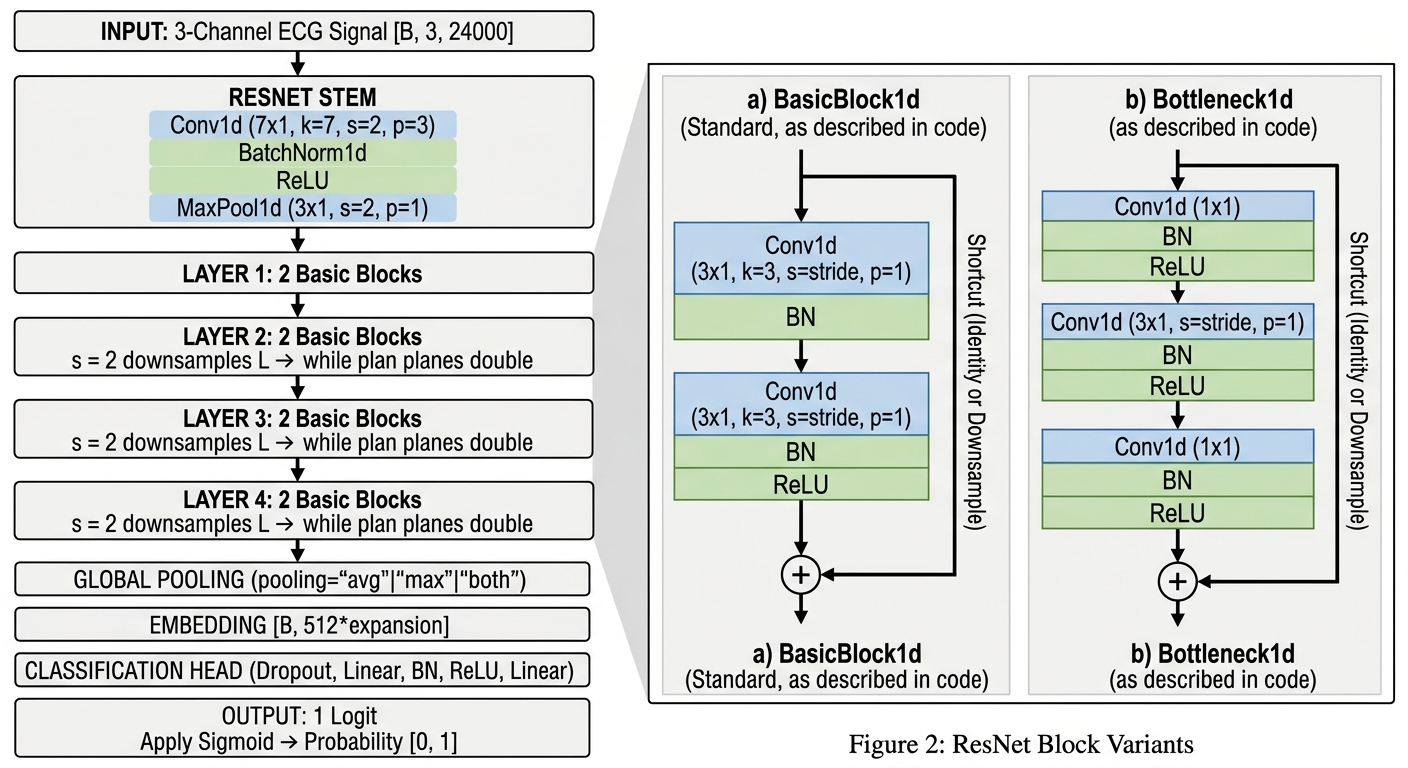
\includegraphics[width=16cm]{figuras/arquitetura_resnet.jpg}}
	}{
		\Fonte{adaptado de \citeonline{he2016deep}.}
	}
\end{figure}

\subsubsection{Bloco básico}
\label{subsubsec:fund-bloco-basico}

O bloco básico é composto por duas convoluções de núcleo $\kappa = 3$, cada
uma seguida de normalização em lote, com ativação \textit{ReLU} após a
primeira e após a soma com o atalho:

\begin{equation}
	\mathcal{F}(\mathbf{x}) = \mathrm{BN}\Big(\mathrm{Conv}_3\big(
	\mathrm{ReLU}(\mathrm{BN}(\mathrm{Conv}_3(\mathbf{x})))\big)\Big),
	\qquad
	\mathbf{y} = \mathrm{ReLU}\big(\mathcal{F}(\mathbf{x}) + \mathbf{x}\big).
	\label{eq:bloco-basico}
\end{equation}

O número de canais na saída é igual ao da camada interna, o que se expressa
por um fator de expansão $E = 1$.

\subsubsection{Bloco de gargalo}
\label{subsubsec:fund-bloco-gargalo}

Em redes mais profundas, o custo de duas convoluções de núcleo três com
muitos canais torna-se proibitivo. O bloco de gargalo substitui-as por três
convoluções: a primeira, de núcleo unitário, reduz o número de canais; a
segunda, de núcleo três, opera sobre a dimensão reduzida; a terceira, também
de núcleo unitário, expande os canais em $E = 4$ vezes. A convolução de
núcleo unitário não considera vizinhança temporal --- combina apenas os
canais em cada posição ---, e é por isso computacionalmente barata.

Para um bloco com 256 canais na entrada e na saída, a versão básica exigiria
$2 \times 256 \times 256 \times 3 \approx 393\,000$ pesos; a de gargalo, com
dimensão interna de 64, exige $256 \times 64 + 64 \times 64 \times 3 + 64
	\times 256 \approx 45\,000$ --- cerca de nove vezes menos. É essa economia
que viabiliza arquiteturas com dezenas de camadas.

\subsection{Arquitetura}
\label{subsec:fund-resnet-arquitetura}

A arquitetura empregada adapta ao domínio unidimensional a estrutura proposta
por \citeonline{he2016deep}, seguindo a prática estabelecida em trabalhos de
classificação de \gls{ECG} com redes residuais
\cite{hannun2019cardiologist,ribeiro2020automatic}. Uma etapa inicial
precede quatro estágios de blocos residuais:

\begin{itemize}
	\item \textbf{Etapa inicial:} convolução com núcleo 7 e passo 2, seguida
	      de normalização em lote, \textit{ReLU} e agrupamento máximo com núcleo 3 e
	      passo 2. O comprimento é reduzido por quatro antes do primeiro bloco.
	\item \textbf{Estágios 1 a 4:} sequências de blocos residuais com $P$,
	      $2P$, $4P$ e $8P$ canais internos, em que $P$ denota a largura inicial.
	      O primeiro bloco dos estágios 2 a 4 emprega passo 2, dividindo o
	      comprimento pela metade e exigindo projeção no atalho.
	\item \textbf{Agrupamento global e classificador:} idênticos aos da
	      \autoref{subsec:fund-cnn-arquitetura}, com o vetor resultante de
	      dimensão $2 \times 8 \cdot P \cdot E$ ao combinar média e máximo.
\end{itemize}

A cada estágio, portanto, o comprimento temporal é dividido por dois e a
profundidade da representação, multiplicada por dois --- progressão distinta
da adotada na rede convolucional da \autoref{sec:fund-cnn}, que divide o
comprimento por quatro a cada bloco.

\subsubsection{Configurações avaliadas}
\label{subsubsec:fund-resnet-config}

Três parâmetros definem cada configuração: o tipo de bloco, o número de
blocos por estágio e a largura inicial $P$. A
\autoref{tab:resnet-configuracoes} reúne as quatro variantes avaliadas, que
percorrem uma faixa de dezesseis vezes em número de parâmetros.

% ---- TABELA: configurações ----
\begin{table}[h!]
	\captionsetup{width=15.5cm}
	\Caption{\label{tab:resnet-configuracoes} Configurações das redes
		residuais avaliadas}
	\IBGEtab{}{
		\begin{tabular}{lcccrr}
			\toprule
			Configuração              & Bloco                          & Blocos por estágio & $P$ &
			\multicolumn{1}{c}{Saída} & \multicolumn{1}{c}{Parâmetros}                                                    \\
			\midrule \midrule
			ResNet-18 reduzida        & básico                         & 2--2--2--2         & 32  & 256    & 1\,029\,985  \\
			ResNet-18 completa        & básico                         & 2--2--2--2         & 64  & 512    & 3\,976\,385  \\
			ResNet-34                 & básico                         & 3--4--6--3         & 64  & 512    & 7\,350\,721  \\
			ResNet-50                 & gargalo                        & 3--4--6--3         & 64  & 2\,048 & 16\,479\,937 \\
			\bottomrule
		\end{tabular}
	}{
		\Fonte{elaborado pelo autor (2026).}
	}
\end{table}

As configurações permitem examinar separadamente duas dimensões da
capacidade. A comparação entre as duas variantes da ResNet-18 isola o efeito
da \textit{largura}: mesma profundidade, o dobro de canais. A comparação
entre a ResNet-18 completa e a ResNet-34 isola o efeito da
\textit{profundidade}: mesma largura, o dobro de blocos. A ResNet-50 combina
a profundidade da ResNet-34 com o bloco de gargalo e saída quatro vezes mais
larga.

Os números de parâmetros são inferiores aos das versões bidimensionais
homônimas, nas quais a ResNet-18 possui cerca de 11 milhões, porque o núcleo
unidimensional de largura três contém três pesos por par de canais, contra
nove do núcleo $3 \times 3$.

\subsubsection{Dimensões e campo receptivo}
\label{subsubsec:fund-resnet-dimensoes}

A \autoref{tab:resnet-dimensoes} apresenta as dimensões das representações
intermediárias para a janela de 24\,000 amostras e o campo receptivo ao
término de cada etapa.

% ---- TABELA: dimensões ----
\begin{table}[h!]
	\captionsetup{width=15.5cm}
	\Caption{\label{tab:resnet-dimensoes} Dimensões e campo receptivo das
		redes residuais para janela de 24\,000 amostras}
	\IBGEtab{}{
		\begin{tabular}{lrrrrr}
			\toprule
			                              &                                 & \multicolumn{2}{c}{Canais} & \multicolumn{2}{c}{Campo receptivo}                     \\
			\cmidrule(lr){3-4} \cmidrule(lr){5-6}
			Etapa                         & \multicolumn{1}{c}{Comprimento} &
			\multicolumn{1}{c}{18 e 34}   & \multicolumn{1}{c}{50}          &
			\multicolumn{1}{c}{ResNet-18} & \multicolumn{1}{c}{ResNet-34}                                                                                          \\
			\midrule \midrule
			Entrada                       & 24\,000                         & 3                          & 3                                   & 5\,ms   & 5\,ms   \\
			Etapa inicial                 & 6\,000                          & 64                         & 64                                  & 55\,ms  & 55\,ms  \\
			Estágio 1                     & 6\,000                          & 64                         & 256                                 & 215\,ms & 295\,ms \\
			Estágio 2                     & 3\,000                          & 128                        & 512                                 & 495\,ms & 895\,ms \\
			Estágio 3                     & 1\,500                          & 256                        & 1\,024                              & 1,1\,s  & 2,7\,s  \\
			Estágio 4                     & 750                             & 512                        & 2\,048                              & 2,2\,s  & 4,5\,s  \\
			\bottomrule
		\end{tabular}
	}{
		\Fonte{elaborado pelo autor (2026).}
	}
\end{table}

O campo receptivo ao final da ResNet-18 é de 2,2\,s --- inferior aos 7,2\,s da
rede convolucional rasa, apesar de esta possuir apenas quatro camadas
convolucionais contra dezessete. A diferença decorre do núcleo: com três
amostras (15\,ms), cada convolução residual amplia pouco a extensão
observada, e a cobertura temporal depende do empilhamento de muitas camadas.
A ResNet-34, com o dobro de blocos, alcança 4,5\,s. A ResNet-50 apresenta
campo receptivo semelhante ao da ResNet-18, pois apenas uma das três
convoluções de cada bloco de gargalo considera vizinhança temporal.

Ainda que inferior à duração da janela, esse campo receptivo não limita a
informação disponível ao classificador: o agrupamento global da
\autoref{eq:pooling-global} combina as 750 posições do último estágio,
abrangendo os dois minutos integralmente.

\subsubsection{Distribuição dos parâmetros}
\label{subsubsec:fund-resnet-parametros}

Os parâmetros concentram-se nos estágios finais, em que o número de canais é
maior. Na ResNet-18 completa, o quarto estágio, com 512 canais, responde por
aproximadamente três quartos do total. Na ResNet-50, o classificador recebe
vetor de 4\,096 dimensões --- 2\,048 de cada agrupamento ---, e sua primeira
camada sozinha possui cerca de 525\,000 parâmetros.

Os pesos das camadas convolucionais são inicializados conforme
\citeonline{he2015delving}, e os parâmetros de escala e deslocamento da
normalização em lote, com um e zero, respectivamente, de modo que cada bloco
inicie próximo da identidade.

\subsection{Considerações sobre o regime de dados}
\label{subsec:fund-resnet-regime}

As redes residuais foram concebidas para conjuntos de treinamento de grande
porte. A ResNet original foi avaliada sobre 1,28 milhão de imagens
\cite{he2016deep}; no domínio do \gls{ECG}, os trabalhos que estabeleceram
seu desempenho empregaram dezenas de milhares a milhões de registros
\cite{hannun2019cardiologist,ribeiro2020automatic}.

Neste trabalho, cada partição dispõe de 309 pacientes no treinamento, dos
quais 33 casos. A razão entre parâmetros e pacientes varia de $3\,333$ na
ResNet-18 reduzida a cerca de $53\,000$ na ResNet-50. Nesse regime, a
capacidade da rede é amplamente suficiente para ajustar individualmente cada
exemplo de treinamento, o que motiva a comparação sistemática entre
configurações de capacidade crescente apresentada no
\autoref{cap:resultados}: se a capacidade fosse o fator limitante, o
desempenho deveria variar com ela.

% ==============================================================================
% FUNDAMENTAÇÃO TEÓRICA — Marcadores eletrocardiográficos
%
% Estrutura:
%   1. Por que marcadores
%   2. Intervalos RR e NN
%   3. Variabilidade da frequência cardíaca: tempo, frequência, não linear
%   4. Morfologia: QRS, QT, QTc
%   5. Ectopia
%   6. Duração do segmento de análise
%
% Notação nova (acrescentar à lista de símbolos):
%   RR_\ell, NN_\ell   \ell-ésimo intervalo RR / NN, em ms
%   n_NN               número de intervalos NN do segmento
%   \overline{NN}      média dos intervalos NN
%   \Delta NN_\ell     diferença entre NN adjacentes
% Siglas: \gls{VFC} (já definida), \gls{ECG}, \gls{MSC}.
% ==============================================================================

% ==============================================================================
% FUNDAMENTAÇÃO TEÓRICA — Mecanismo de atenção
% Baseado na classe ResNetTransformer (resnet_classificacao.py)
%
% Configuração verificada pela contagem de parâmetros (1.491.553, idêntica à
% registrada no log de execução):
%   corpo     ResNet-18 reduzida, sem a cabeça         963.936
%   atenção   1 camada, d=256, 4 cabeças, ff=512       527.104
%   cabeça    Dropout + Linear(512 -> 1)                   513
%
% ⚠️ CONFERIR: o texto afirma que não há codificação posicional, conforme a
%    versão do código escrita durante o projeto. Se ela tiver sido
%    acrescentada depois, ajustar a subseção correspondente.
% ==============================================================================

\section{Mecanismo de atenção}
\label{sec:fund-atencao}

As arquiteturas descritas nas seções anteriores relacionam instantes do
sinal por meio de operações locais. Cada convolução combina apenas $\kappa$
posições vizinhas, e a relação entre instantes distantes só se estabelece
indiretamente, pelo empilhamento de camadas --- daí o campo receptivo de
2,2\,s ao final da ResNet-18, inferior à janela de dois minutos analisada.

O mecanismo de atenção adota princípio distinto: cada posição da sequência
pode ser relacionada diretamente a qualquer outra, em uma única operação,
com intensidade aprendida a partir dos próprios dados. Proposto no contexto
da tradução automática \cite{vaswani2017attention}, tornou-se o componente
central das arquiteturas denominadas \textit{Transformer}.

\subsection{Autoatenção}
\label{subsec:fund-autoatencao}

Seja $\mathbf{X} \in \mathbb{R}^{L \times d}$ uma sequência de $L$ posições,
cada uma representada por um vetor de dimensão $d$. A autoatenção projeta
essa sequência em três matrizes, por meio de transformações lineares
aprendidas:

\begin{equation}
	\mathbf{Q} = \mathbf{X}\mathbf{U}_Q, \qquad
	\mathbf{K} = \mathbf{X}\mathbf{U}_K, \qquad
	\mathbf{V} = \mathbf{X}\mathbf{U}_V,
	\label{eq:qkv}
\end{equation}

\noindent
denominadas consultas, chaves e valores. A saída é obtida ponderando os
valores pela similaridade entre consultas e chaves:

\begin{equation}
	\mathrm{Atenção}(\mathbf{Q}, \mathbf{K}, \mathbf{V}) =
	\mathrm{softmax}\!\left(\frac{\mathbf{Q}\mathbf{K}^{\top}}{\sqrt{d_k}}\right)
	\mathbf{V},
	\label{eq:atencao}
\end{equation}

\noindent
em que $d_k$ é a dimensão das consultas e chaves. O produto
$\mathbf{Q}\mathbf{K}^{\top}$ resulta em matriz $L \times L$ cujo elemento
$(t, s)$ mede o quanto a posição $t$ deve considerar a posição $s$. A função
\textit{softmax}, aplicada a cada linha, converte essas similaridades em
pesos não negativos que somam um. A divisão por $\sqrt{d_k}$ evita que, em
dimensões elevadas, os produtos internos assumam magnitudes que saturariam a
\textit{softmax} e anulariam seus gradientes.

Cada posição da saída é, portanto, uma média ponderada das representações
de todas as posições da sequência, com pesos que dependem do conteúdo. No
contexto do \gls{ECG}, isso permite, em princípio, que a representação de um
batimento incorpore informação de batimentos distantes cujo padrão seja
relevante --- uma extrassístole e a pausa que a sucede, por exemplo.

\subsubsection{Atenção com múltiplas cabeças}
\label{subsubsec:fund-multicabeca}

Em vez de uma única operação de atenção, a formulação usual executa $h$
operações em paralelo, cada uma com projeções próprias de dimensão
$d_k = d/h$, e concatena os resultados:

\begin{equation}
	\mathrm{MultiCabeça}(\mathbf{X}) =
	\big[\mathrm{cabeça}_1; \ldots; \mathrm{cabeça}_h\big]\,\mathbf{U}_O,
	\qquad
	\mathrm{cabeça}_i = \mathrm{Atenção}\big(\mathbf{X}\mathbf{U}_Q^{(i)},
	\mathbf{X}\mathbf{U}_K^{(i)}, \mathbf{X}\mathbf{U}_V^{(i)}\big).
	\label{eq:multicabeca}
\end{equation}

Cada cabeça pode especializar-se em um tipo de relação --- uma em vizinhança
imediata, outra em padrões periódicos, por exemplo ---, sem que o custo total
seja superior ao de uma única cabeça de dimensão $d$.

\subsection{Camada codificadora}
\label{subsec:fund-codificador}

A camada codificadora do \textit{Transformer} combina a atenção com
múltiplas cabeças e uma rede totalmente conectada aplicada a cada posição
separadamente, ambas envolvidas por conexões residuais e normalização:

\begin{align}
	\mathbf{X}' &= \mathrm{LN}\big(\mathbf{X} + \mathrm{MultiCabeça}(\mathbf{X})\big),
	\label{eq:codificador-1} \\
	\mathbf{Y} &= \mathrm{LN}\big(\mathbf{X}' + \mathrm{FFN}(\mathbf{X}')\big),
	\label{eq:codificador-2}
\end{align}

\noindent
em que $\mathrm{FFN}$ é composta por duas camadas lineares com ativação
intermediária, a primeira expandindo a dimensão de $d$ para $d_{\mathrm{ff}}$
e a segunda restaurando-a. As conexões residuais desempenham o mesmo papel
discutido na \autoref{subsec:fund-residual}.

A normalização empregada é a normalização de camada \cite{ba2016layer},
que padroniza cada vetor individualmente, ao longo de suas $d$ dimensões, em
lugar de cada canal ao longo do lote como na
\autoref{eq:batchnorm}. A escolha torna a operação independente do tamanho
do lote e do comprimento da sequência.

\subsection{Custo computacional}
\label{subsec:fund-atencao-custo}

A matriz de atenção possui $L^2$ elementos por cabeça, e o custo da operação
cresce com o quadrado do comprimento da sequência. Esse aspecto determina
onde a atenção pode ser inserida em arquiteturas para sinais longos.

Aplicada diretamente à janela de 24\,000 amostras, a atenção exigiria matriz
de $576$ milhões de elementos por cabeça e por exemplo --- volume
incompatível com o processamento em lote. Aplicada após o corpo
convolucional, que reduz a sequência a 750 posições, a matriz passa a ter
$562\,500$ elementos, redução de aproximadamente mil vezes. A combinação de
camadas convolucionais seguidas de atenção explora essa complementaridade:
as convoluções extraem padrões locais e comprimem a sequência, e a atenção
relaciona os padrões resultantes ao longo de toda a janela.

\subsection{Arquitetura empregada}
\label{subsec:fund-atencao-arquitetura}

A arquitetura avaliada mantém integralmente o corpo da ResNet-18 reduzida
(\autoref{tab:resnet-configuracoes}), que produz sequência de 750 posições
com 256 canais, e insere entre ele e o agrupamento global uma camada
codificadora com os parâmetros da \autoref{tab:atencao-config}.

% ---- TABELA: configuração ----
\begin{table}[h!]
	\captionsetup{width=12cm}
	\Caption{\label{tab:atencao-config} Configuração da camada de atenção}
	\IBGEtab{}{
		\begin{tabular}{ll}
			\toprule
			Parâmetro & Valor \\
			\midrule \midrule
			Comprimento da sequência ($L$) & 750 posições \\
			Dimensão do modelo ($d$) & 256 \\
			Número de cabeças ($h$) & 4 \\
			Dimensão por cabeça ($d_k$) & 64 \\
			Dimensão da rede interna ($d_{\mathrm{ff}}$) & 512 \\
			Número de camadas & 1 \\
			Descarte & 0,3 \\
			\bottomrule
		\end{tabular}
	}{
	\Fonte{elaborado pelo autor (2026).}
}
\end{table}

A saída do codificador, com as mesmas dimensões da entrada, passa pelo
agrupamento global combinado de média e máximo, resultando em vetor de 512
dimensões. Diferentemente das demais redes, o classificador consiste em uma
única camada linear precedida de descarte, sem camada intermediária: a
capacidade adicional introduzida pela atenção dispensa a não linearidade
extra no classificador.

A \autoref{tab:atencao-parametros} decompõe os parâmetros.

% ---- TABELA: parâmetros ----
\begin{table}[h!]
	\captionsetup{width=12.5cm}
	\Caption{\label{tab:atencao-parametros} Distribuição dos parâmetros da
	ResNet-18 reduzida com camada de atenção}
	\IBGEtab{}{
		\begin{tabular}{lrr}
			\toprule
			Componente & \multicolumn{1}{c}{Parâmetros} &
			\multicolumn{1}{c}{Fração} \\
			\midrule \midrule
			Corpo residual & 963\,936 & 64,6\,\% \\
			Atenção com múltiplas cabeças & 263\,168 & 17,6\,\% \\
			Rede interna (FFN) & 262\,912 & 17,6\,\% \\
			Normalização de camada & 1\,024 & 0,1\,\% \\
			Classificador & 513 & $<$\,0,1\,\% \\
			\midrule
			Total & 1\,491\,553 & 100,0\,\% \\
			\bottomrule
		\end{tabular}
	}{
	\Fonte{elaborado pelo autor (2026).}
}
\end{table}

A camada de atenção acrescenta $527\,104$ parâmetros, cerca de metade do
corpo convolucional e 35\,\% do total.

\subsubsection{Ausência de codificação posicional}
\label{subsubsec:fund-posicional}

A operação da \autoref{eq:atencao} é invariante à ordem das posições: se a
sequência de entrada for permutada, a saída é permutada da mesma forma. Em
aplicações nas quais a ordem é essencial, como a linguagem, acrescenta-se à
entrada uma \textit{codificação posicional} que identifica cada posição
\cite{vaswani2017attention}.

A arquitetura empregada não utiliza codificação posicional. Duas razões
sustentam a escolha. A primeira é que as representações produzidas pelo
corpo convolucional já carregam informação local de ordem, pois cada posição
resume um trecho contíguo do sinal. A segunda é que a saída do codificador é
submetida ao agrupamento global, operação também invariante à ordem: a
posição absoluta de um padrão dentro da janela de dois minutos não altera a
representação final. O que a atenção acrescenta, nesse arranjo, é a
possibilidade de cada posição ser representada em função do conteúdo das
demais, e não a modelagem da ordem temporal propriamente dita.

\subsection{Considerações sobre o regime de dados}
\label{subsec:fund-atencao-regime}

As arquiteturas baseadas em atenção apresentam menos vieses indutivos que
as convolucionais. Uma convolução pressupõe, por construção, que padrões
relevantes são locais e podem ocorrer em qualquer posição; a atenção não
pressupõe localidade e precisa aprender, a partir dos dados, quais relações
são relevantes. \citeonline{dosovitskiy2021image} mostraram que essa
flexibilidade só se converte em vantagem quando o conjunto de treinamento é
suficientemente grande: em conjuntos de pequeno porte, modelos baseados em
atenção apresentaram desempenho inferior ao de redes convolucionais de
capacidade semelhante.

A arquitetura híbrida aqui empregada atenua esse problema ao preservar o
corpo convolucional e restringir a atenção a uma única camada sobre
representações já comprimidas. Ainda assim, com 33 casos positivos por
partição de treinamento, a estimativa dos $527\,104$ parâmetros adicionais
encontra-se no regime em que a literatura reporta menor eficácia do
mecanismo.

\section{Marcadores eletrocardiográficos}
\label{sec:fund-marcadores}

As redes neurais descritas nas seções anteriores aprendem diretamente do
sinal quais padrões são relevantes para a tarefa. A alternativa clássica
inverte essa ordem: calculam-se do \gls{ECG} medidas com significado
fisiológico conhecido, e um modelo estatístico simples relaciona essas
medidas ao desfecho. Essas medidas são chamadas, neste trabalho, de
\textit{marcadores eletrocardiográficos}; na literatura, recebem também os
nomes de biomarcadores digitais ou de métricas derivadas do \gls{ECG}.

A abordagem tem duas vantagens em uma coorte pequena. A primeira é a
economia de parâmetros: cada marcador condensa milhares de amostras do sinal
em um único número, e um modelo com poucas dezenas de coeficientes pode ser
ajustado com 55 eventos sem memorizar os pacientes de treinamento. A segunda
é a interpretabilidade: cada coeficiente refere-se a um mecanismo
fisiológico identificável --- o controle autonômico do ritmo, a duração da
repolarização ventricular, a frequência de batimentos ectópicos ---, o que
permite confrontar os resultados com o conhecimento clínico. Em
contrapartida, o modelo só tem acesso à informação que os marcadores
escolhidos capturam; padrões do sinal que não correspondam a nenhum deles
são descartados.

Os marcadores empregados pertencem a três grupos: a variabilidade da
frequência cardíaca, a morfologia do batimento e a ectopia. Todos partem da
mesma etapa inicial, a localização dos picos R.

\subsection{Intervalos RR e intervalos NN}
\label{subsec:fund-rr-nn}

O pico R é o ponto de maior amplitude do complexo QRS e marca a
despolarização ventricular de cada batimento. Detectados os picos, o
intervalo $\mathrm{RR}_\ell$\glsadd{RR}\glsunset{RR} é o tempo, em milissegundos, entre o
$\ell$-ésimo pico e o seguinte. A sequência de intervalos RR descreve a
frequência cardíaca batimento a batimento e é a matéria-prima de todos os
marcadores de ritmo.

Nem todo intervalo RR reflete, porém, a modulação normal do ritmo sinusal.
Um batimento ectópico --- originado fora do nó sinusal --- produz um
intervalo curto seguido de outro longo; um pico não detectado produz um
intervalo com aproximadamente o dobro da duração esperada; um artefato
detectado como pico produz dois intervalos curtos. A diretriz da
\textit{Task Force} \cite{taskforce1996heart} estabelece, por isso, que os
marcadores de variabilidade sejam calculados apenas sobre intervalos entre
batimentos sinusais normais, chamados intervalos NN\glsadd{NN}\glsunset{NN}. Na prática, um
intervalo é considerado normal quando não se afasta mais que uma fração
pré-definida da mediana dos intervalos vizinhos. Um único batimento
ectópico em um segmento curto pode multiplicar o valor de alguns marcadores,
como se mostra na \autoref{sec:met-extracao}.

A distinção é especialmente importante neste trabalho, que procura nos
batimentos ectópicos um sinal de risco. Os intervalos que não são NN não
são descartados da análise: eles deixam de entrar nos marcadores de
variabilidade, mas passam a compor os marcadores de ectopia descritos na
\autoref{subsec:fund-ectopia}.

\subsection{Variabilidade da frequência cardíaca}
\label{subsec:fund-vfc}

A frequência cardíaca de um indivíduo saudável em repouso não é constante.
Ela oscila continuamente sob a ação do sistema nervoso autônomo: o ramo
parassimpático, mediado pelo nervo vago, produz variações rápidas,
acopladas à respiração; o ramo simpático, variações mais lentas. A
\gls{VFC} quantifica essas oscilações e funciona, assim, como uma medida
indireta do equilíbrio autonômico. Na insuficiência cardíaca, a ativação
simpática persistente e a retirada vagal reduzem a \gls{VFC}. A redução da
\gls{VFC} está associada a maior mortalidade desde os primeiros estudos com
Holter, realizados em pacientes após infarto do miocárdio
\cite{kleiger1987decreased}.

\subsubsection{Domínio do tempo}

Os marcadores do domínio do tempo são estatísticas calculadas diretamente
sobre a sequência de $n_{\mathrm{NN}}$ intervalos NN de um segmento. O \gls{SDNN},

\begin{equation}
	\mathrm{SDNN} = \sqrt{\frac{1}{n_{\mathrm{NN}} - 1}
		\sum_{\ell=1}^{n_{\mathrm{NN}}}
		\left( \mathrm{NN}_\ell - \overline{\mathrm{NN}} \right)^2},
	\label{eq:sdnn}
\end{equation}

\noindent
em que $\overline{\mathrm{NN}}$ é a média dos intervalos, reflete a
variabilidade total do segmento, somando as componentes rápidas e lentas.
A \gls{RMSSD},

\begin{equation}
	\mathrm{RMSSD} = \sqrt{\frac{1}{n_{\mathrm{NN}} - 1}
		\sum_{\ell=1}^{n_{\mathrm{NN}} - 1} \left( \Delta \mathrm{NN}_\ell \right)^2},
	\qquad
	\Delta \mathrm{NN}_\ell = \mathrm{NN}_{\ell+1} - \mathrm{NN}_\ell,
	\label{eq:rmssd}
\end{equation}

\noindent
e o \gls{pNN50},
isolam as variações de um batimento para o seguinte e são, por isso,
associados predominantemente à modulação vagal. A diferença
$\Delta \mathrm{NN}_\ell$ só tem significado quando os dois intervalos são
adjacentes no registro: se um batimento ectópico foi removido entre eles, a
diferença compararia intervalos que não se sucederam, e não entra no
cálculo.

\subsubsection{Domínio da frequência}

A análise espectral decompõe a variância dos intervalos em faixas de
frequência associadas a mecanismos distintos \cite{taskforce1996heart}. A
faixa de \gls{HF}, de 0,15 a 0,4\,Hz, corresponde à arritmia
sinusal respiratória e à modulação vagal; a de \gls{LF}, de 0,04 a 0,15\,Hz, a uma combinação de influências simpáticas e vagais
ligadas ao barorreflexo; a de \gls{VLF}, abaixo de 0,04\,Hz, a mecanismos mais lentos, como a termorregulação. A razão LF/HF
é frequentemente interpretada como índice do balanço simpatovagal, embora
essa leitura seja controversa.

A estimativa espectral impõe uma duração mínima ao segmento. Um ciclo de
0,04\,Hz, limite inferior da faixa LF, dura 25\,s, e uma estimativa estável
da potência nessa faixa exige que vários ciclos estejam contidos no
segmento. A \textit{Task Force} recomenda segmentos de pelo menos 2~minutos
para a faixa LF e de 5~minutos como padrão para a análise espectral de
curta duração \cite{taskforce1996heart}.

\subsubsection{Medidas não lineares}

O gráfico de Poincaré representa cada intervalo NN contra o seguinte. A
dispersão dos pontos perpendicularmente à diagonal, SD1\glsadd{SD1}\glsunset{SD1}, mede a
variabilidade de curto prazo; a dispersão ao longo da diagonal, SD2\glsadd{SD2}\glsunset{SD2}, a de
longo prazo \cite{brennan2001poincare}. Ambas podem ser obtidas das
variâncias já definidas:

\begin{equation}
	\mathrm{SD1} = \sqrt{\tfrac{1}{2}\,\mathrm{Var}(\Delta \mathrm{NN})},
	\qquad
	\mathrm{SD2} = \sqrt{2\,\mathrm{Var}(\mathrm{NN}) -
		\tfrac{1}{2}\,\mathrm{Var}(\Delta \mathrm{NN})}.
	\label{eq:poincare}
\end{equation}

\noindent
A primeira expressão mostra que SD1 é proporcional ao \gls{RMSSD} e carrega,
portanto, a mesma informação. A razão SD1/SD2 descreve a forma da nuvem de
pontos e é menos redundante em relação aos demais marcadores.

A entropia amostral mede a regularidade da sequência de intervalos: valores
baixos indicam uma série previsível, e valores altos, uma série complexa
\cite{richman2000physiological}. Por depender da contagem de padrões
repetidos, ela exige sequências de centenas de batimentos para ser
estimada com estabilidade.

\subsection{Morfologia do batimento}
\label{subsec:fund-morfologia}

Os marcadores de morfologia descrevem a forma do batimento, e não o
intervalo entre batimentos. Sua obtenção exige delinear cada batimento,
isto é, localizar o início, o pico e o fim das ondas P, QRS e T.

A \textit{duração do QRS} mede o tempo de despolarização dos ventrículos.
Seu prolongamento indica condução intraventricular lenta, como nos bloqueios
de ramo, e está associado a pior prognóstico na insuficiência cardíaca. O
\textit{intervalo QT}\glsadd{QT}\glsunset{QT}, do início do QRS ao fim da onda T, abrange a
despolarização e a repolarização ventriculares. Como o QT encurta
naturalmente quando a frequência cardíaca aumenta, ele é comparado entre
pacientes após correção pela frequência. A correção de Bazett
\cite{bazett1920analysis} divide o QT pela raiz quadrada do intervalo RR
expresso em segundos:

\begin{equation}
	\mathrm{QTc} = \frac{\mathrm{QT}}{\sqrt{\overline{\mathrm{RR}}}}.
	\label{eq:bazett}
\end{equation}

\noindent
O prolongamento do QTc\glsadd{QTc}\glsunset{QTc} reflete repolarização ventricular lenta ou
heterogênea, substrato conhecido para arritmias ventriculares.

A delineação automática é a etapa menos robusta da extração. As fronteiras
das ondas não têm definição única, os algoritmos divergem entre si, e o
ruído do Holter --- registrado durante as atividades diárias do paciente ---
desloca as marcações. Por isso, as durações obtidas automaticamente devem
ser entendidas como estimativas consistentes dentro de um mesmo método, e
não como medidas comparáveis aos valores de referência clínicos.

\subsection{Ectopia}
\label{subsec:fund-ectopia}

Um batimento ectópico ocorre antes do esperado e, quando de origem
ventricular, costuma ser seguido de uma pausa compensatória. As
extrassístoles ventriculares frequentes e, sobretudo, as sequências de dois
ou mais batimentos ectópicos consecutivos são reconhecidas como marcadores
de instabilidade elétrica na insuficiência cardíaca.

A identificação definitiva da origem de um batimento exige a análise de sua
morfologia. Na ausência dessa análise, a ectopia pode ser aproximada pelo
ritmo: um intervalo RR muito mais curto que os vizinhos indica um batimento
precoce; um intervalo curto seguido de um longo, uma extrassístole com
pausa compensatória; dois intervalos curtos consecutivos, um duplete. Essa
aproximação não distingue a origem ventricular da supraventricular e deve
ser descrita como um indicador de ectopia, e não como uma contagem de
extrassístoles ventriculares.

\subsection{Duração do segmento de análise}
\label{subsec:fund-duracao-segmento}

Os marcadores não são calculados sobre o Holter inteiro, mas sobre
segmentos, e a duração do segmento determina quais deles podem ser
estimados. A \autoref{tab:fund-duracao-marcadores} resume essa relação.
Segmentos curtos permitem acompanhar a evolução dos marcadores ao longo do
dia, mas restringem o conjunto calculável e aumentam a variância de cada
estimativa: com cerca de 35 batimentos em 30~segundos, um único intervalo
anômalo pesa sobre o \gls{SDNN} e o \gls{RMSSD} muito mais que em 5~minutos.

\begin{table}[h!]
	\captionsetup{width=14cm}
	\Caption{\label{tab:fund-duracao-marcadores} Marcadores calculáveis em
		segmentos de 5 minutos e de 30 segundos}
	\IBGEtab{}{
		\begin{tabular}{lcc}
			\toprule
			Marcador                      & 5 minutos                    & 30 segundos              \\
			\midrule \midrule
			SDNN, RMSSD, pNN50, SD1, SD2  & sim                          & sim, com maior variância \\
			Potência LF, HF e razão LF/HF & sim                          & não                      \\
			Potência VLF                  & não (exige registros longos) & não                      \\
			Entropia amostral             & sim                          & não                      \\
			QRS, QT, QTc                  & sim                          & sim                      \\
			Indicadores de ectopia        & sim                          & sim                      \\
			\bottomrule
		\end{tabular}
	}{
		\Fonte{elaborado pelo autor (2026), com base em
			\citeonline{taskforce1996heart}.}
	}
\end{table}

Como cada paciente contribui com dezenas ou centenas de segmentos, os
valores precisam ser resumidos em uma única linha por paciente antes da
modelagem, pelas razões discutidas na \autoref{subsec:fund-agregacao}. O
resumo pode descrever o nível típico de cada marcador, por exemplo pela
mediana, e também sua variação ao longo do registro, que reflete a
modulação circadiana e a instabilidade do controle autonômico.

A \autoref{tab:fund-biomarcadores} reúne os marcadores extraídos neste
trabalho, com sua definição, unidade e significado fisiológico. Cada um é
calculado em cada segmento e depois resumido por paciente de duas formas: a
média entre os segmentos, que representa o nível típico do marcador, e o
desvio-padrão entre os segmentos, que representa quanto ele varia ao longo
do dia. Assim, o desvio-padrão da frequência cardíaca média, por exemplo, não
mede a variação batimento a batimento, mas a diferença de frequência entre os
períodos do registro, incluindo o ciclo dia--noite.

\begin{table}[h!]
	\captionsetup{width=16cm}
	\Caption{\label{tab:fund-biomarcadores} Marcadores eletrocardiográficos
		extraídos: definição e significado}
	\IBGEtab{}{
		\footnotesize
		\begin{tabular}{p{3.3cm}p{5.6cm}p{1.1cm}p{5.2cm}}
			\toprule
			Marcador & Definição & Unidade & Significado \\
			\midrule \midrule
			\multicolumn{4}{l}{\textit{Ritmo e variabilidade (sobre intervalos NN)}} \\
			Frequência cardíaca média & 60\,000 dividido pela média dos intervalos NN & bpm & Nível de ativação do ritmo \\
			Intervalo RR médio & Média dos intervalos NN & ms & Inverso da frequência \\
			\gls{SDNN} & Desvio-padrão dos intervalos NN (\autoref{eq:sdnn}) & ms & Variabilidade total do segmento \\
			\gls{RMSSD} & Raiz da média dos quadrados das diferenças sucessivas (\autoref{eq:rmssd}) & ms & Variação batimento a batimento; tônus vagal \\
			\gls{pNN50} & Porcentagem de diferenças sucessivas maiores que 50\,ms & \% & Tônus vagal \\
			SD1 e SD2 & Dispersões do gráfico de Poincaré (\autoref{eq:poincare}) & ms & Variabilidade de curto e de longo prazo \\
			SD1/SD2 & Razão entre as duas dispersões & --- & Forma da nuvem de Poincaré \\
			\gls{VLF}, \gls{LF}, \gls{HF}, LF/HF & Potência espectral por faixa (só em 5~minutos) & ms$^2$ & Modulação autonômica por mecanismo \\
			Entropia amostral & Regularidade da sequência de intervalos (só em 5~minutos) & --- & Complexidade do ritmo \\
			\midrule
			\multicolumn{4}{l}{\textit{Ectopia e pausas (pelo ritmo, sem distinguir a origem)}} \\
			Batimentos precoces & Intervalos RR menores que 80\,\% da mediana local & contagem & Batimentos fora do ritmo sinusal \\
			Extrassístoles & Precoce seguido de intervalo maior que 115\,\% da mediana local & contagem & Batimento ectópico com pausa compensatória \\
			Dupletes & Dois intervalos precoces consecutivos & contagem & Ectopia repetitiva; instabilidade elétrica \\
			Carga de ectopia & Porcentagem de intervalos precoces & \% & Frequência global de ectopia \\
			Intervalos irregulares & Porcentagem de intervalos plausíveis que não são NN & \% & Irregularidade do ritmo \\
			Maior pausa & Maior intervalo RR plausível do segmento & ms & Pausas e bradiarritmias \\
			Pausas acima de 2\,s & Intervalos RR maiores que 2\,000\,ms & contagem & Pausas prolongadas \\
			\midrule
			\multicolumn{4}{l}{\textit{Morfologia (mediana dos batimentos delineados)}} \\
			Duração do QRS & Do início ao fim do complexo QRS & ms & Condução ventricular; bloqueios de ramo \\
			Intervalo \gls{QT} & Do início do QRS ao fim da onda T & ms & Despolarização e repolarização ventriculares \\
			\gls{QTc} & QT corrigido pela frequência (\autoref{eq:bazett}) & ms & Repolarização prolongada; risco arrítmico \\
			Ondas P e T identificadas & Fração dos batimentos com cada onda delineada & --- & Qualidade do sinal e da delineação \\
			Amplitude & Percentil 99 do valor absoluto do sinal filtrado, por derivação & mV & Massa ventricular ativa e geometria \\
			\bottomrule
		\end{tabular}
	}{
		\Fonte{elaborado pelo autor (2026), com base em
			\citeonline{taskforce1996heart}.}
	}
\end{table}




% ==============================================================================
% FUNDAMENTAÇÃO TEÓRICA — Métricas e avaliação de classificadores
%
% Estrutura:
%   1. Matriz de confusão e métricas dependentes de limiar
%   2. Curva ROC e AUC
%   3. Curva precisão-revocação e AP
%   4. Escolha do limiar (índice de Youden)
%   5. Agregação por paciente
%   6. Validação cruzada estratificada por paciente
%   7. Intervalos de confiança e comparação de modelos (bootstrap)
%
% Notação: conforme notacao_dissertacao.md
%   y_i rótulo   \hat{p}_i probabilidade estimada   \delta limiar
%   C_1, C_0 conjuntos de casos e controles   \varphi comparação de um par
%   M_i janelas do paciente i   J índice de Youden   B^* reamostragens
%   N_1 positivos   N_0 negativos   \pi prevalência
% Siglas já definidas: AUC, AP, VPP, MSC, ECG.
% Siglas novas usadas por extenso: VPN, ROC (acrescentar \newacronym se preferir).
% ==============================================================================

\section{Modelos tabulares e aprendizado de representações}
\label{sec:fund-tabulares}

Os marcadores e as variáveis clínicas formam uma tabela, com uma linha por
paciente e uma coluna por variável. Esta seção descreve os modelos ajustados
sobre essas tabelas e duas formas de obter, a partir do sinal, colunas
adicionais aprendidas por uma rede neural.

\subsection{Regressão logística regularizada}
\label{subsec:fund-logistica}

A regressão logística estima a probabilidade de evento de um paciente com
variáveis $\mathbf{x}$ como

\begin{equation}
	p(\mathbf{x}) = \sigma\!\left(\beta_0 + \boldsymbol{\beta}^{\top}\mathbf{x}\right),
	\label{eq:reg-logistica}
\end{equation}

\noindent
em que $\sigma$ é a função logística (\autoref{eq:logistica}). Com as
variáveis padronizadas, $e^{\beta_j}$ é a razão de chances associada ao
aumento de um desvio-padrão na variável $j$. Os coeficientes são obtidos
minimizando a entropia cruzada acrescida de uma penalização: a penalização
L2, $\lambda \lVert \boldsymbol{\beta} \rVert_2^2$, encolhe todos os
coeficientes sem anulá-los; a penalização L1,
$\lambda \lVert \boldsymbol{\beta} \rVert_1$, anula parte deles e realiza,
portanto, seleção de variáveis. Com poucos eventos, a penalização reduz o
sobreajuste, mas não o elimina: a regra usual de dez eventos por variável
\cite{peduzzi1996simulation} indica que, com 33 casos de treinamento, um
modelo confiável comporta poucas variáveis, o que favorece conjuntos
pequenos definidos antes de olhar os dados.

\subsection{Análise de componentes principais}
\label{subsec:fund-pca}

Quando há muitas variáveis correlacionadas, a \gls{PCA} as substitui por
poucas combinações lineares não correlacionadas, ordenadas pela variância
que explicam. As direções são estimadas apenas com os pacientes de
treinamento e aplicadas, sem alteração, aos de teste. Neste trabalho, a
\gls{PCA} reduz os 128 valores da representação de uma rede a oito
componentes antes da regressão logística.

\subsection{Aprendizado multitarefa com rótulos substitutos}
\label{subsec:fund-multitarefa}

Quando o desfecho de interesse é raro, uma rede pode ser treinada em outras
tarefas, com rótulos abundantes e relacionados ao problema, chamados rótulos
substitutos. No aprendizado multitarefa \cite{caruana1997multitask}, um
mesmo extrator $f_{\theta}$ alimenta $K$ saídas, uma por tarefa, e a perda
total é a média das perdas individuais:

\begin{equation}
	\mathcal{L} = \frac{1}{\sum_k w_k m_k} \sum_{k=1}^{K} w_k\, m_k\, \ell_k\!\left(\hat{y}_k, y_k\right),
	\label{eq:multitarefa}
\end{equation}

\noindent
em que $\ell_k$ é o erro quadrático para tarefas contínuas ou a entropia
cruzada para tarefas binárias, $w_k$ é o peso da tarefa e $m_k$ vale zero
quando o rótulo está ausente. Para prever bem todas as tarefas, o extrator
precisa produzir uma \textit{representação}
$\mathbf{z} = f_{\theta}(\mathbf{s})$ --- o vetor da penúltima camada --- que
resuma o que há de comum entre elas. Essa representação é depois usada como
variável de um modelo pequeno, ajustado ao desfecho raro.

\subsection{Aprendizado autossupervisionado}
\label{subsec:fund-autossupervisionado}

No aprendizado autossupervisionado, os rótulos são gerados a partir do
próprio sinal, sem nenhuma anotação externa. No aprendizado contrastivo
\cite{chen2020simple}, duas visões de um mesmo objeto formam um par positivo,
e as demais visões do lote, pares negativos. Para \gls{ECG},
\citeonline{kiyasseh2021clocs} propuseram usar como par positivo dois
trechos do mesmo paciente. Com representações normalizadas
$\mathbf{u}_i$ e $\mathbf{u}_j$ de um par positivo, a perda é

\begin{equation}
	\ell_{ij} = -\log \frac{\exp(\mathbf{u}_i^{\top}\mathbf{u}_j/\tau)}
	{\sum_{k \neq i} \exp(\mathbf{u}_i^{\top}\mathbf{u}_k/\tau)},
	\label{eq:nt-xent}
\end{equation}

\noindent
em que $\tau$ é a temperatura. Alternativamente, um \textit{autoencoder}
comprime o sinal em uma representação de dimensão reduzida e o reconstrói,
minimizando o erro quadrático; na variante mascarada, parte do sinal é
apagada e a rede precisa reconstruí-la a partir do contexto. Em todos os
casos, nada garante que os padrões aprendidos tenham relação com o desfecho:
a rede tende a capturar as fontes de variação mais fortes do sinal, que
podem ser alheias ao risco.

\section{Avaliação de classificadores binários}
\label{sec:fund-metricas}

Um classificador binário, como as redes e os modelos logísticos deste
trabalho, produz para cada paciente $i$ uma probabilidade estimada
$\hat{p}_i \in [0, 1]$ de pertencer à classe positiva --- neste trabalho, o
óbito por \gls{MSC}. Avaliar o classificador significa medir o quanto essas
probabilidades separam os pacientes que sofreram o evento dos que não o
sofreram. Esta seção apresenta as métricas empregadas, distinguindo as que
dependem de um limiar de decisão das que avaliam a ordenação das
probabilidades, e descreve os procedimentos usados para estimar a incerteza
dessas métricas em uma amostra pequena e desbalanceada.

\subsection{Matriz de confusão e métricas dependentes de limiar}
\label{subsec:fund-confusao}

Para converter a probabilidade em uma decisão, fixa-se um limiar $\delta$: o
paciente é classificado como positivo se $\hat{p}_i \geq \delta$ e como
negativo caso contrário. O cruzamento entre a classe predita e a classe real
gera os quatro desfechos da matriz de confusão, apresentada na
\autoref{tab:fund-confusao}.

\begin{table}[h!]
	\captionsetup{width=12cm}
	\Caption{\label{tab:fund-confusao} Matriz de confusão de um
		classificador binário}
	\IBGEtab{}{
		\begin{tabular}{lcc}
			\toprule
			                        & Predito positivo         & Predito negativo         \\
			\midrule \midrule
			Real positivo ($y = 1$) & Verdadeiro positivo (VP) & Falso negativo (FN)      \\
			Real negativo ($y = 0$) & Falso positivo (FP)      & Verdadeiro negativo (VN) \\
			\bottomrule
		\end{tabular}
	}{
		\Fonte{elaborado pelo autor (2026).}
	}
\end{table}

A partir dessas contagens definem-se as métricas da
\autoref{tab:fund-metricas-limiar}. A sensibilidade e a especificidade
descrevem o desempenho dentro de cada classe real e não dependem da
proporção entre as classes. O \gls{VPP} e o valor preditivo negativo (VPN),
ao contrário, respondem à pergunta clínica --- dado o resultado do
classificador, qual a probabilidade de o paciente estar na classe indicada
--- e por isso dependem da prevalência $\pi$ do evento na população
avaliada.

\begin{table}[h!]
	\captionsetup{width=15cm}
	\Caption{\label{tab:fund-metricas-limiar} Métricas derivadas da matriz
		de confusão}
	\IBGEtab{}{
		\begin{tabular}{lcl}
			\toprule
			Métrica                   & Definição                                                                          & Interpretação \\
			\midrule \midrule
			Sensibilidade (revocação) & $\dfrac{\mathrm{VP}}{\mathrm{VP} + \mathrm{FN}}$                                   &
			fração dos óbitos identificada                                                                                                 \\[2ex]
			Especificidade            & $\dfrac{\mathrm{VN}}{\mathrm{VN} + \mathrm{FP}}$                                   &
			fração dos sobreviventes corretamente descartada                                                                               \\[2ex]
			\gls{VPP} (precisão)      & $\dfrac{\mathrm{VP}}{\mathrm{VP} + \mathrm{FP}}$                                   &
			probabilidade de óbito entre os sinalizados                                                                                    \\[2ex]
			VPN                       & $\dfrac{\mathrm{VN}}{\mathrm{VN} + \mathrm{FN}}$                                   &
			probabilidade de sobrevida entre os não sinalizados                                                                            \\[2ex]
			Acurácia                  & $\dfrac{\mathrm{VP} + \mathrm{VN}}{N}$                                             &
			fração total de acertos                                                                                                        \\[2ex]
			F1                        & $\dfrac{2 \cdot \mathrm{VPP} \cdot \mathrm{Sens.}}{\mathrm{VPP} + \mathrm{Sens.}}$ &
			média harmônica entre \gls{VPP} e sensibilidade                                                                                \\
			\bottomrule
		\end{tabular}
	}{
		\Fonte{elaborado pelo autor (2026).}
	}
\end{table}

A acurácia merece cautela em problemas desbalanceados. Com prevalência de
10,6\,\%, um classificador que declare todos os pacientes sobreviventes
alcança acurácia de 89,4\,\% sem identificar nenhum óbito. Pelo mesmo motivo,
o \gls{VPP} deve ser lido em relação à prevalência: um \gls{VPP} próximo de
$\pi$ indica que ser sinalizado pelo classificador pouco altera a
probabilidade de óbito em relação à da coorte como um todo.

Todas essas métricas dependem do limiar escolhido. Reduzir $\delta$ aumenta a
sensibilidade à custa da especificidade, e vice-versa, de modo que um único
par de valores descreve apenas um ponto de operação do classificador. Por
esse motivo, a métrica principal deste trabalho é independente de limiar.

\subsection{Curva ROC e área sob a curva}
\label{subsec:fund-roc}

A curva ROC\glsadd{ROC}\glsunset{ROC} (\textit{Receiver Operating Characteristic}) representa o
classificador em todos os limiares possíveis simultaneamente: para cada
$\delta$, marca-se a taxa de verdadeiros positivos (sensibilidade) contra a
taxa de falsos positivos ($1 -$ especificidade) \cite{fawcett2006introduction}.
Um classificador sem capacidade discriminativa produz a diagonal que liga
$(0, 0)$ a $(1, 1)$; um classificador perfeito passa pelo ponto $(0, 1)$.

A \gls{AUC} resume a curva em um único número e admite uma interpretação
probabilística direta \cite{hanley1982meaning}: é a probabilidade de que um
paciente sorteado entre os que sofreram o evento receba probabilidade
estimada maior que um paciente sorteado entre os que não o sofreram. Com
$N_1$ positivos e $N_0$ negativos, ela é estimada por

\begin{equation}
	\mathrm{AUC} = \frac{1}{N_1 N_0}
	\sum_{i \in \mathcal{C}_1} \sum_{j \in \mathcal{C}_0}
	\varphi\!\left(\hat{p}_i, \hat{p}_j\right),
	\qquad
	\varphi(a, b) =
	\begin{cases}
		1,            & a > b, \\
		\tfrac{1}{2}, & a = b, \\
		0,            & a < b,
	\end{cases}
	\label{eq:auc}
\end{equation}

\noindent
em que $\mathcal{C}_1$ e $\mathcal{C}_0$ são os conjuntos de casos e de
controles, com $N_1$ e $N_0$ elementos. A função $\varphi$ compara um caso
$i$ com um controle $j$ e vale 1 quando o caso recebeu a maior
probabilidade. A \gls{AUC} é, portanto, a fração dos $N_1 N_0$ pares em que
o caso foi ordenado acima do controle: 0,5 corresponde à ordenação aleatória
e 1,0 à separação perfeita.

Duas propriedades tornam a \gls{AUC} adequada como métrica principal deste
trabalho. Ela não depende de limiar, o que permite comparar modelos
independentemente do ponto de operação escolhido. E ela não depende da
prevalência, já que cada par contém exatamente um caso e um controle, o que
a torna comparável entre coortes com proporções diferentes de eventos. Em
contrapartida, a \gls{AUC} mede apenas a ordenação: um modelo pode ter
\gls{AUC} elevada e, ainda assim, produzir probabilidades mal calibradas ou
um \gls{VPP} baixo quando o evento é raro.

\subsection{Curva precisão-revocação e precisão média}
\label{subsec:fund-ap}

Quando a classe positiva é rara, a curva ROC pode transmitir uma impressão
otimista: como a taxa de falsos positivos é calculada sobre os numerosos
negativos, um número absoluto elevado de falsos positivos pode corresponder a
uma taxa pequena. A curva precisão-revocação contorna esse efeito ao
relacionar o \gls{VPP} à sensibilidade, concentrando-se no desempenho sobre a
classe positiva \cite{saito2015precision, davis2006relationship}.

A \gls{AP} resume essa curva como a média ponderada do \gls{VPP} obtido em
cada limiar, com pesos iguais ao incremento de sensibilidade:

\begin{equation}
	\mathrm{AP} = \sum_{q} \left( \mathrm{Sens}_q - \mathrm{Sens}_{q-1} \right) \mathrm{VPP}_q,
	\label{eq:ap}
\end{equation}

\noindent
em que $\mathrm{VPP}_q$ e $\mathrm{Sens}_q$ são o \gls{VPP} e a sensibilidade
no $q$-ésimo limiar, percorridos em ordem decrescente. Diferentemente da \gls{AUC}, a \gls{AP}
depende da prevalência: o valor de referência de um classificador aleatório
não é 0,5, mas a própria prevalência $\pi$, igual a 0,106 nesta coorte. Uma
\gls{AP} só indica capacidade discriminativa quando supera esse valor.

\subsection{Escolha do limiar de decisão}
\label{subsec:fund-youden}

As métricas da \autoref{tab:fund-metricas-limiar} exigem que um limiar seja
fixado. Neste trabalho, o limiar é o que maximiza o índice de Youden
\cite{youden1950index}:

\begin{equation}
	J(\delta) = \mathrm{Sensibilidade}(\delta) + \mathrm{Especificidade}(\delta) - 1,
	\qquad
	\delta^{*} = \arg\max_{\delta} J(\delta).
	\label{eq:youden}
\end{equation}

\noindent
Geometricamente, $\delta^{*}$ corresponde ao ponto da curva ROC mais distante
da diagonal. O critério atribui o mesmo peso a sensibilidade e
especificidade, o que é apropriado quando não se fixou previamente o custo
relativo de um falso negativo e de um falso positivo.

O limiar é um parâmetro ajustado aos dados e, como tal, deve ser escolhido
sem acesso ao conjunto de teste. Escolhê-lo sobre os mesmos pacientes em que
as métricas são reportadas produziria estimativas otimistas de sensibilidade
e especificidade. Por isso, $\delta^{*}$ é determinado no conjunto de validação
interna de cada partição e aplicado, sem alteração, ao conjunto de teste
correspondente.

\subsection{Agregação por paciente}
\label{subsec:fund-agregacao}

As redes neurais deste trabalho não recebem o Holter inteiro, mas janelas
extraídas dele, e produzem uma probabilidade para cada janela. O rótulo, por
outro lado, pertence ao paciente. Calcular as métricas sobre janelas
trataria como observações independentes centenas de trechos do mesmo exame,
que compartilham o mesmo rótulo e são fortemente correlacionados entre si.
O tamanho amostral efetivo seria superestimado, e os intervalos de confiança
resultantes, estreitos demais --- um caso de pseudorreplicação.

Por esse motivo, toda métrica é calculada no nível do paciente. A
probabilidade do paciente $i$ é a média das probabilidades de suas $M_i$
janelas:

\begin{equation}
	\hat{p}_i = \frac{1}{M_i} \sum_{m=1}^{M_i} \hat{p}_{i,m},
	\label{eq:agregacao-paciente}
\end{equation}

\noindent
em que $\hat{p}_{i,m}$ é a probabilidade estimada para a $m$-ésima janela. A
média reflete o risco típico ao longo do registro e é menos sensível a
janelas isoladas com artefato do que alternativas como o máximo.

\subsection{Validação cruzada estratificada por paciente}
\label{subsec:fund-validacao-cruzada}

Com 517 pacientes e 55 eventos, separar um único conjunto de teste deixaria
cerca de uma dezena de casos para a avaliação, e o resultado dependeria
fortemente de quais pacientes fossem sorteados. A validação cruzada em $K$
partições reduz essa dependência: os pacientes são divididos em $K$ grupos
disjuntos, e cada grupo é usado uma vez como teste enquanto os demais formam
o treinamento \cite{kohavi1995study}. Ao final, cada paciente recebe
exatamente uma predição feita por um modelo que não o viu durante o
treinamento --- a predição \textit{fora da partição}.

Dois cuidados são essenciais nesse procedimento. O primeiro é a
\textit{estratificação}: as partições são formadas de modo que a proporção de
eventos seja aproximadamente a mesma em todas, o que evita partições com
pouquíssimos casos. O segundo é a \textit{separação por paciente}: todas as
janelas de um mesmo exame pertencem à mesma partição. Se janelas de um
paciente estivessem simultaneamente no treinamento e no teste, o modelo
poderia reconhecer o indivíduo, e não o padrão associado ao desfecho,
inflando as métricas. Esse tipo de vazamento de informação está entre os
erros mais frequentes em estudos de aprendizado de máquina aplicado
\cite{kapoor2023leakage}.

Pelo mesmo princípio, todo procedimento que aprende a partir dos dados ---
imputação de valores ausentes, padronização, cálculo da escala do sinal,
redução de dimensionalidade e escolha do limiar --- é ajustado apenas com os
pacientes de treinamento de cada partição e então aplicado ao teste.

\subsection{Intervalos de confiança e comparação entre modelos}
\label{subsec:fund-bootstrap}

Uma \gls{AUC} estimada em 517 pacientes, dos quais 55 positivos, está sujeita
a variabilidade amostral considerável, e reportá-la sem intervalo de
confiança impediria distinguir um resultado de outro ou do acaso. Os
intervalos foram obtidos por \textit{bootstrap} \cite{efron1993introduction}.
O procedimento sorteia, com reposição, $N$ pacientes entre os $N$ da coorte,
recalcula a métrica sobre essa reamostra a partir das predições fora da
partição e repete o processo $B^{*}$ vezes. O intervalo de confiança de 95\,\%
é formado pelos percentis 2,5 e 97,5 da distribuição das $B^{*}$ estimativas.
O valor de $B^{*}$ adotado em cada experimento é informado na metodologia.

O intervalo oferece um critério direto de comparação com o acaso: se ele
contém 0,5, o desempenho do classificador não é distinguível de uma
ordenação aleatória dos pacientes.

Comparar dois modelos exige um cuidado adicional. Como ambos são avaliados
sobre os mesmos pacientes, suas \gls{AUC} são correlacionadas, e comparar
intervalos calculados separadamente seria conservador. Emprega-se, por isso,
o \textit{bootstrap} pareado: em cada reamostra, calcula-se a diferença
\begin{equation}
	\Delta_b = \mathrm{AUC}_b^{(1)} - \mathrm{AUC}_b^{(2)}, \qquad b = 1, \dots, B^{*},
	\label{eq:delta-auc}
\end{equation}
\noindent
sobre o mesmo conjunto de pacientes sorteados, e o intervalo de confiança da
diferença é obtido pelos percentis da distribuição de $\Delta_b$. O modelo
1 é considerado superior ao modelo 2 apenas se esse intervalo não contiver zero.

% Alguns autores preferem fazer uma ``fundamentação teórica'' no segundo capítulo, outros, preferem fazer uma ``revisão da literatura''. Entretanto, isto é particular de cada trabalho e o autor deve escolher o título mais adequado para o capítulo. Consultar o orientador é importante para determinar o título apropriado.

% Evite começar da seção secundária, ou seja, não passe direto do título do capítulo para o título da seção secundária. Escreva um texto para introduzir as seções subsequentes. Lembre-se de utilizar primeira letra maiúscula quando estiver se referindo a um objeto com numeração específica como capítulo, seção, subseção, figura, tabela, quadro, equação, normalmente, se escreve a primeira letra maiúscula da palavra do objeto seguido do \textit{label}. Por exemplo, a Seção \ref{sec:citacoes} explica como fazer citações bibliográficas. Observe no código fonte deste texto como foi feita a referência cruzada. Isso permite enumerar a seção do modo automático o que facilita caso novas seções sejam criadas.

% \section{Citações bibliográficas}\label{sec:citacoes}

% Esta frase mostra como citar um livro sobre descargas atmosféricas \cite{rakov2003lightning}. Também podem ser citados \textit{sites} como \citeonline{elat2015densidade}. Você precisa escrever o código da referência no arquivo "referencia.bib" dentro da pasta "elementos-pos-textuais". Veja esse, onde estão alguns exemplos que já foram testados.

% Referenciando outro livro \cite{LangtangenLogg2017}. Texto texto texto texto texto texto texto texto texto texto texto texto texto texto texto texto texto texto texto. Texto texto texto texto texto texto texto texto texto texto texto texto texto texto texto texto texto texto texto. Texto texto texto texto texto texto texto texto texto texto texto texto texto texto texto texto texto texto texto. Texto texto texto texto texto texto texto texto texto texto texto texto texto texto texto texto texto texto texto.

% Referenciando outro site \cite{secretaria1999}. Texto texto texto texto texto texto texto texto texto texto texto texto texto texto texto texto texto texto texto. Texto texto texto texto texto texto texto texto texto texto texto texto texto texto texto texto texto texto texto. Texto texto texto texto texto texto texto texto texto texto texto texto texto texto texto texto texto texto texto. Texto texto texto texto texto texto texto texto texto texto texto texto texto texto texto texto texto texto texto. Citando uma norma \cite{NBR10520:2002}.

% Citação de duas referências que concordam entre si \cite{Almeida2018,Gondim2017}. Texto texto texto texto texto texto texto texto texto texto texto texto texto texto texto texto texto texto texto. Texto texto texto texto texto texto texto texto texto texto texto texto texto texto texto texto texto texto texto. Texto texto texto texto texto texto texto texto texto texto texto texto texto texto texto texto texto texto texto. Texto texto texto texto texto texto texto texto texto texto texto texto texto texto texto texto texto texto texto texto texto texto texto texto texto texto. Citando um manual \cite{manuais1989}.

% Outro tipo de citação é a citação literal ou direta com mais de três linhas. Este tipo de citação deve ser destacada com recuo de $4~cm$ da margem esquerda com letra menor (tamanho 10), sem aspas e com espaçamento simples.  Para exemplificar esse tipo de citação, considere a afirmação de \citeonline{feitosa2016}:
% \begin{citacao}
% 	A cultura é o processo através do qual o homem cria o algo onde antes imperava o nada. Esse algo é toda complexidade de criações simbólicas, de sentidos e significados que damos às coisas e ao mundo. Um ``algo'' que não se sustenta se não se entender os processos culturais como mecanismos de mediação entre nós e os fenômenos. Assim, mais do que apenas um elemento da comunicação, a mediação é, por excelência, cultural. As diversas modalidades de mediação são apenas sotaques diferenciados dessa mediação cultural. Assim é a mediação informacional.
% \end{citacao}

% A afirmação do parágrafo anterior também pode ser reproduzida com a citação na final como mostra o exemplo a seguir:
% \begin{citacao}
% 	A cultura é o processo através do qual o homem cria o algo onde antes imperava o nada. Esse algo é toda complexidade de criações simbólicas, de sentidos e significados que damos às coisas e ao mundo. Um “algo” que não se sustenta se não se entender os processos culturais como mecanismos de mediação entre nós e os fenômenos. Assim, mais do que apenas um elemento da comunicação, a mediação é, por excelência, cultural. As diversas modalidades de mediação são apenas sotaques diferenciados dessa mediação cultural. Assim é a mediação informacional. \cite{feitosa2016}.
% \end{citacao}

% %Mais exemplos e opções de citações podem ser encontradas em:
% %        https://en.wikibooks.org/wiki/LaTeX/Bibliography_Management
% %        https://github.com/cfgnunes/latex-cefetmg/blob/master/latex-cefetmg/03-elementos-pos-textuais/apendices.tex            

% \section{Inserindo figuras}\label{sec:figuras}

% A Figura \ref{fig:reitoria} apresenta a fotografia da reitoria da Universidade Federal do Ceará. Observe a estrutura do código para ver como inserir figuras. No título, comece especificando o tipo de figura. Por exemplo, fotografia, desenho, diagrama, fluxograma, gráfico e etc. O espaçamento entre linhas no título é de $1~pt$ (espaçamento simples), apenas a primeira letra da frase é maiúscula. As demais palavras são escritas com letra maiúsculas somente quando são nomes próprios e não há ponto final.

% As margens do título da figura são delimitadas pelo tamanho da figura. Por isso, procure ajustar o tamanho da figura para preencher a largura delimitada pelas margens esquerda e direita da página que possui $16~cm$ de largura. Não esqueça de indicar fonte da figura. O autor deve evitar deixar figuras pequenas menores do que $7~cm$ de largura.

% A posição da figura deve ser o mais próximo logo após ter sido chamada no texto (a figura nunca deve aparecer antes de ter sido anunciada no texto).

% %troque h pelo b ou t para mudar a posição da figura.
% \begin{figure}[h!]
% 	\captionsetup{width=16cm}%Da mesma largura que a figura
% 	\Caption{\label{fig:reitoria} Fotografia da reitoria da Universidade Federal do Ceará}
% 	\UFCfig{}{
% 		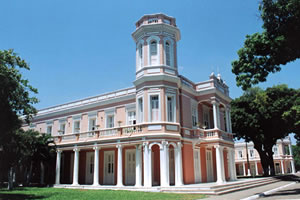
\includegraphics[width=16cm]{figuras/exemplo-1}
% 	}{
% 		\Fonte{\citeonline{UFC2012}.}
% 	}
% \end{figure}

% Texto1 texto texto texto texto texto texto texto texto texto texto texto texto texto texto texto texto texto texto texto texto texto texto texto texto texto texto texto texto texto texto texto texto texto texto texto texto texto texto texto texto texto texto texto texto1.

% Texto2 texto texto texto texto texto texto texto texto texto texto texto texto texto texto texto texto texto texto. Texto texto texto texto texto texto texto texto texto texto texto texto texto texto texto texto texto texto texto2.

% Texto3 texto texto texto texto texto texto texto texto texto texto texto texto texto texto texto texto texto texto. Texto texto texto texto texto texto texto texto texto texto texto texto texto texto texto texto texto texto texto3.

% Texto4 texto texto texto texto texto texto texto texto texto texto texto texto texto texto texto texto texto texto. Texto texto texto texto texto texto texto texto texto texto texto texto texto texto texto texto texto texto texto4.

% A Figura \ref{fig:sondas} Texto texto texto texto texto texto texto texto texto texto texto texto texto texto texto texto texto texto texto. Texto texto texto texto texto texto texto texto texto texto texto texto texto texto texto texto texto texto texto3.

% \begin{figure}[h!]
% 	\centering
% 	\captionsetup{width=14cm}%Da mesma largura que a figura
% 	\Caption{\label{fig:sondas} Gráfico da Atmosfera Superior}
% 	\UFCfig{}{
% 		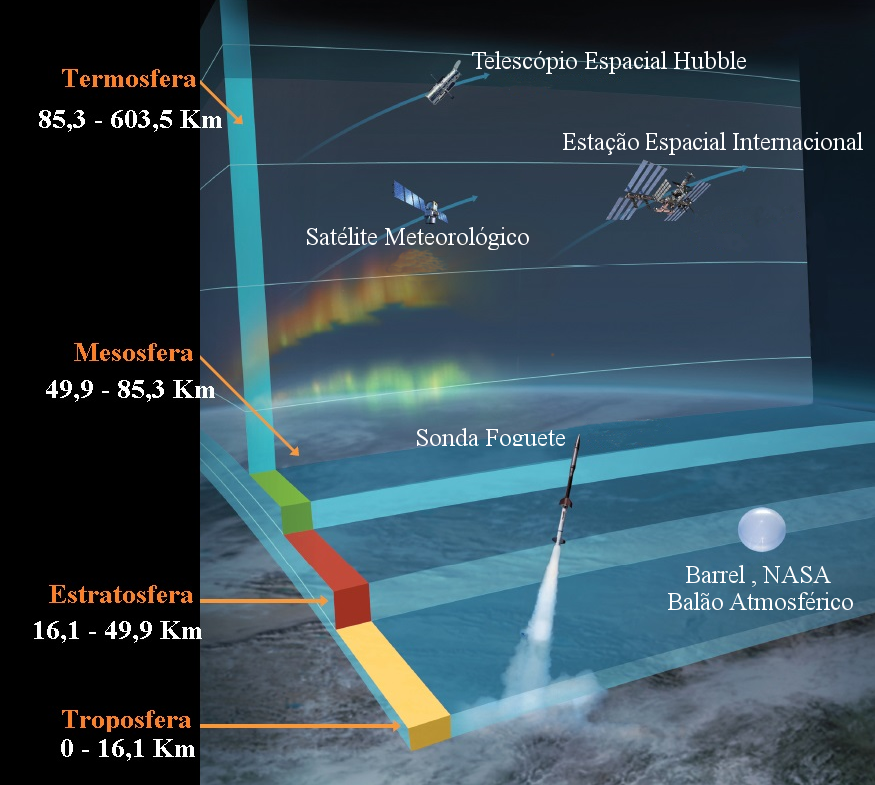
\includegraphics[width=14cm]{figuras/sondas}
% 	}{
% 		\Fonte{adaptado da \citeonline{NASA2016}.}}
% \end{figure}

% Texto5 texto texto texto texto texto texto texto texto texto texto texto texto texto texto texto texto texto texto texto texto texto texto texto texto texto texto texto texto texto texto texto texto texto texto texto texto texto texto texto texto texto texto texto texto5.

% Texto6 texto texto texto texto texto texto texto texto texto texto texto texto texto texto texto texto texto texto texto texto texto texto texto texto texto texto texto texto texto texto texto texto texto texto texto texto texto texto texto texto texto texto texto texto5.

% Texto7 texto texto texto texto texto texto texto texto texto texto texto texto texto texto texto texto texto texto texto texto texto texto texto texto texto texto texto texto texto texto texto texto texto texto texto texto texto texto texto texto texto texto texto texto texto texto texto texto texto texto texto texto texto texto texto texto texto texto texto texto texto texto texto6.

% Evite terminar seções, capítulos e etc com figura. Procure escrever mais.

% \section{Inserindo tabelas}\label{sec:tabelas}

% A Tabela \ref{tab:exemplo-1}... texto texto texto texto texto texto texto texto texto texto texto texto texto texto texto texto texto texto texto. Texto texto texto texto texto texto texto texto texto texto texto texto texto texto texto texto texto texto texto.

% \begin{table}[!h]
% 	\captionsetup{width=7cm}%Deixe da mesma largura que a tabela
% 	\Caption{\label{tab:exemplo-1} Um Exemplo de tabela alinhada que pode ser longa ou curta}%
% 	\IBGEtab{}{%
% 		\begin{tabular}{ccc}
% 			\toprule
% 			Nome           & Nascimento & Documento      \\
% 			\midrule \midrule
% 			Maria da Silva & 11/11/1111 & 111.111.111-11 \\
% 			Maria da Silva & 11/11/1111 & 111.111.111-11 \\
% 			Maria da Silva & 11/11/1111 & 111.111.111-11 \\
% 			\bottomrule
% 		\end{tabular}%
% 	}{%
% 		\Fonte{o autor.}%
% 		\Nota{esta é uma nota, que diz que os dados são baseados na
% 			regressão linear.}%
% 		\Nota[Anotações]{uma anotação adicional, seguida de várias outras.}%
% 	}
% \end{table}

% %\begin{table}[h!]	
% %	\centering
% %	\Caption{\label{tab:exemplo-1} Exemplo de tabela}	
% %	\UFCtab{}{
% %		\begin{tabular}{cll}
% %			\toprule
% %			Ranking & Exon Coverage & Splice Site Support \\
% %			\midrule \midrule
% %			E1 & Complete coverage by a single transcript & Both splice sites\\
% %			E2 & Complete coverage by more than a single transcript & Both splice sites\\
% %			E3 & Partial coverage & Both splice sites\\
% %			E4 & Partial coverage & One splice site\\
% %			E5 & Complete or partial coverage & No splice sites\\
% %			E6 & No coverage & No splice sites\\
% %			\bottomrule
% %		\end{tabular}
% %	}{
% %	\Fonte{elaborado pelo autor.}
% %}
% %\end{table}

% \subsection{Exemplo de subseção} \label{sec:ex_sec}

% Texto texto texto texto texto texto texto texto texto texto texto texto texto texto texto texto texto texto texto texto texto texto texto texto texto texto texto texto texto texto texto texto texto texto texto texto texto texto texto texto texto texto texto texto texto.

% %acrlong{DATASUS},\acrlong{DNV},\acrlong{DO},\acrlong{ESF},\acrlong{IBGE},\acrlong{MFC},\acrlong{MI},\acrlong{MS},\acrlong{NV},\acrlong{ODM},\acrlong{OI},\acrlong{OMS},\acrlong{ONU},\acrlong{PNI},\acrlong{PSF},\acrlong{RIPSA},\acrlong{RN},\acrlong{SIM},\acrlong{SINASC},\acrlong{SUS},\acrlong{TMI},\acrlong{TMMFC}


% \begin{alineascomponto}
% 	\item Integer non lacinia magna. Aenean tempor lorem tellus, non sodales nisl commodo ut
% 	\item Proin mattis placerat risus sit amet laoreet. Praesent sapien arcu, maximus ac fringilla efficitur, vulputate faucibus sem. Donec aliquet velit eros, sit amet elementum dolor pharetra eget
% 	\item Integer eget mattis libero. Praesent ex velit, pulvinar at massa vel, fermentum dictum mauris. Ut feugiat accumsan augue, et ultrices ipsum euismod vitae
% 	\begin{subalineascomponto}
% 		\item Integer non lacinia magna. Aenean tempor lorem tellus, non sodales nisl commodo ut
% 		\item Proin mattis placerat risus sit amet laoreet.
% 	\end{subalineascomponto}
% \end{alineascomponto}

% \subsection{Uso de siglas} \label{sec:siglas}

% Para utilizar siglas, primeiro defina a sigla no arquivo "lista-de-abreviaturas-e-siglas"~ dentro da pasta "1-pre-textuais" com o comando
% \begin{verbatim}
%         \newacronym{ABNT}{ABNT}{Associação Brasileira de Normas Técnicas}
%     \end{verbatim}
% Depois chame a sigla com o comando:
% \begin{verbatim}
%         \gls{ABNT}
%     \end{verbatim}
% Fica assim: \gls{ABNT}. A primeira vez que o comando é usado para uma determinada sigla, aparece o significado por extenso da sigla com a sua abreviação em seguida. A partir da segunda vez que o comando para uma determinada sigla é usado, aparace apenas a sigla. Por exemplo: \gls{ABNT}.

% Veja o código fonte de outros exemplos: Teste de siglas \gls{TEST}, outros exemplos de siglas: \gls{DA}, \gls{MCEG}.
% Repare que sempre as siglas estão sendo definidas primeiramente no arquivo ``lista-de-abreviaturas-e-siglas''.